\chapter{Double-CPA laser architecture}
\label{chapter:Overall presentation of the laser system}
\minitoc
\thispagestyle{empty}

The laser system in Salle Noire is a sub-TW system delivering a few mJ, 30fs, Carrier Envelope Phase (CEP) controlled, high-contrast beam at 1kHz~\cite{Jullien}. TW-class lasers and above often operate at a lower repetition rate, typically in the Hz range \cite{yanovsky2008ultra,malka2002electron,loupias2007plasma}. However, in laser-plasma interaction schemes,  it is very common that users operate in single shot mode regardless of the laser repetition rate (e.g a mechanical shutter) because thermal effects in the laser chain usually degrade the laser performance or simply because other operations, like moving the target to refresh the target surface require more time than available between two successive laser shots \cite{quere2008phase}. Compared to other installations where high-intensity laser-plasma experiments are conducted, our laser has a relatively low peak-power (<TW) so that thermal effects can be efficiently managed for a continuous operation at 1kHz. A high intensity ($\sim 10^{18}\,\mathrm{W/cm^2}$) on target is reached by focusing the laser with a parabola of very short focal length (f = $52\,\mathrm{mm}$) while a stable rotating target developed by Antonin Borot during his PhD\cite{theseAnto} enables the surface to be refreshed every millisecond.

\section{Global architecture}
\subsection{Overview of the laser chain}
Extensive details on the laser system can be found in \cite{TheseRicci,TheseTrisorio,TheseCanova}, and a schematic representation is given in Fig~\ref{fig:femtopower}. We present here the main constituent blocks of the laser system from the "front-end" towards the solid-target experimental chamber. \\

%Inside the Femtopower, we have the oscillator, the vary fist block of the laser system, followed by a 10 pass CPA amplifier.\\

\noindent \g{First CPA (Chirped Pulse Amplifier):} The first block of the laser chain, also called front-end, is a commercial Titanium:Sapphire (Ti:Sa) stabilized laser from \textit{Femtolaser GmbH}~\cite{moulton1986spectroscopic}: the oscillator generates a train of  $\sim$nJ pulses at a frequency of $80\,\mathrm{MHz}$. The pulse is then stretched to $\sim 20\,\mathrm{ps}$ with a SF57 bulk stretcher and sent into a 10-pass amplifier (first CPA of the laser chain). After 4 passes, the train frequency is reduced to 1kHz with a Pockels cell. In the end, the front-end delivers 1.8mJ, 30fs CEP stable pulses with a contrast of $10^{8}$.\\
\noindent \g{XPW:} After this first CPA, the beam is injected into an "XPW contrast filter" (described more in details in \ref{subsection:XPW contrast cleaning}) which function is to enhance the temporal contrast of the pulse through a degenerate four-wave mixing process~\cite{jullien200510}.\\
\noindent \g{Laser stretching before second CPA:}
Dispersive propagation in 75cm of SF57 bulk material stretches the laser from roughly 30fs to 45ps. \\
\g{Dazzler:}
The Dazzler is a commercial acousto-optic modulator (\textit{Fastlite})~\cite{verluise2000amplitude} used to shape the temporal properties of the incoming laser pulse. Through a user interface, it is possible to linearly shape the spectrum and the phase (decomposed on a polynomial base) of the beam. This 
module is extremely convenient to finely adjust the compression of the pulse on target.\\
\noindent \g{Second CPA :} The stretched pulse is then amplified with two consecutive Ti-Sa power amplifiers pumped with a frequency doubled Nd:Yag (\textit{Photonics Industry}).\\
 \g{Compression:} After amplification, the beam is partially compressed in air with set of grisms (\textit{Fastlite}) chosen because they can compensate the third-order phase introduced by the bulk stretcher. The beam is then focused into a hollow core fiber under vacuum, which filters the beam spatial profile. After the fiber, the beam is recollimated with a spherical mirror and separated into a "main pulse" and a "prepulse" with a beam splitter. The final compression of both pulses is done in the "beam compression" vacuum chamber to avoid non-linear effects in the entrance window, using a set of chirped mirrors. \\
 \g{Target chamber:}  After compression, the beam is expanded by a factor 3 with a telescope to reach the tight focus regime ($f/1.2$) and sent to the experimental solid-target chamber,  located at the end of the laser chain. Both main pulse and prepulse are focused on target using the same off-axis parabola. Its full description is given in \ref{section:Solid target experimental set-up}.





\begin{figure}[H]
\centering
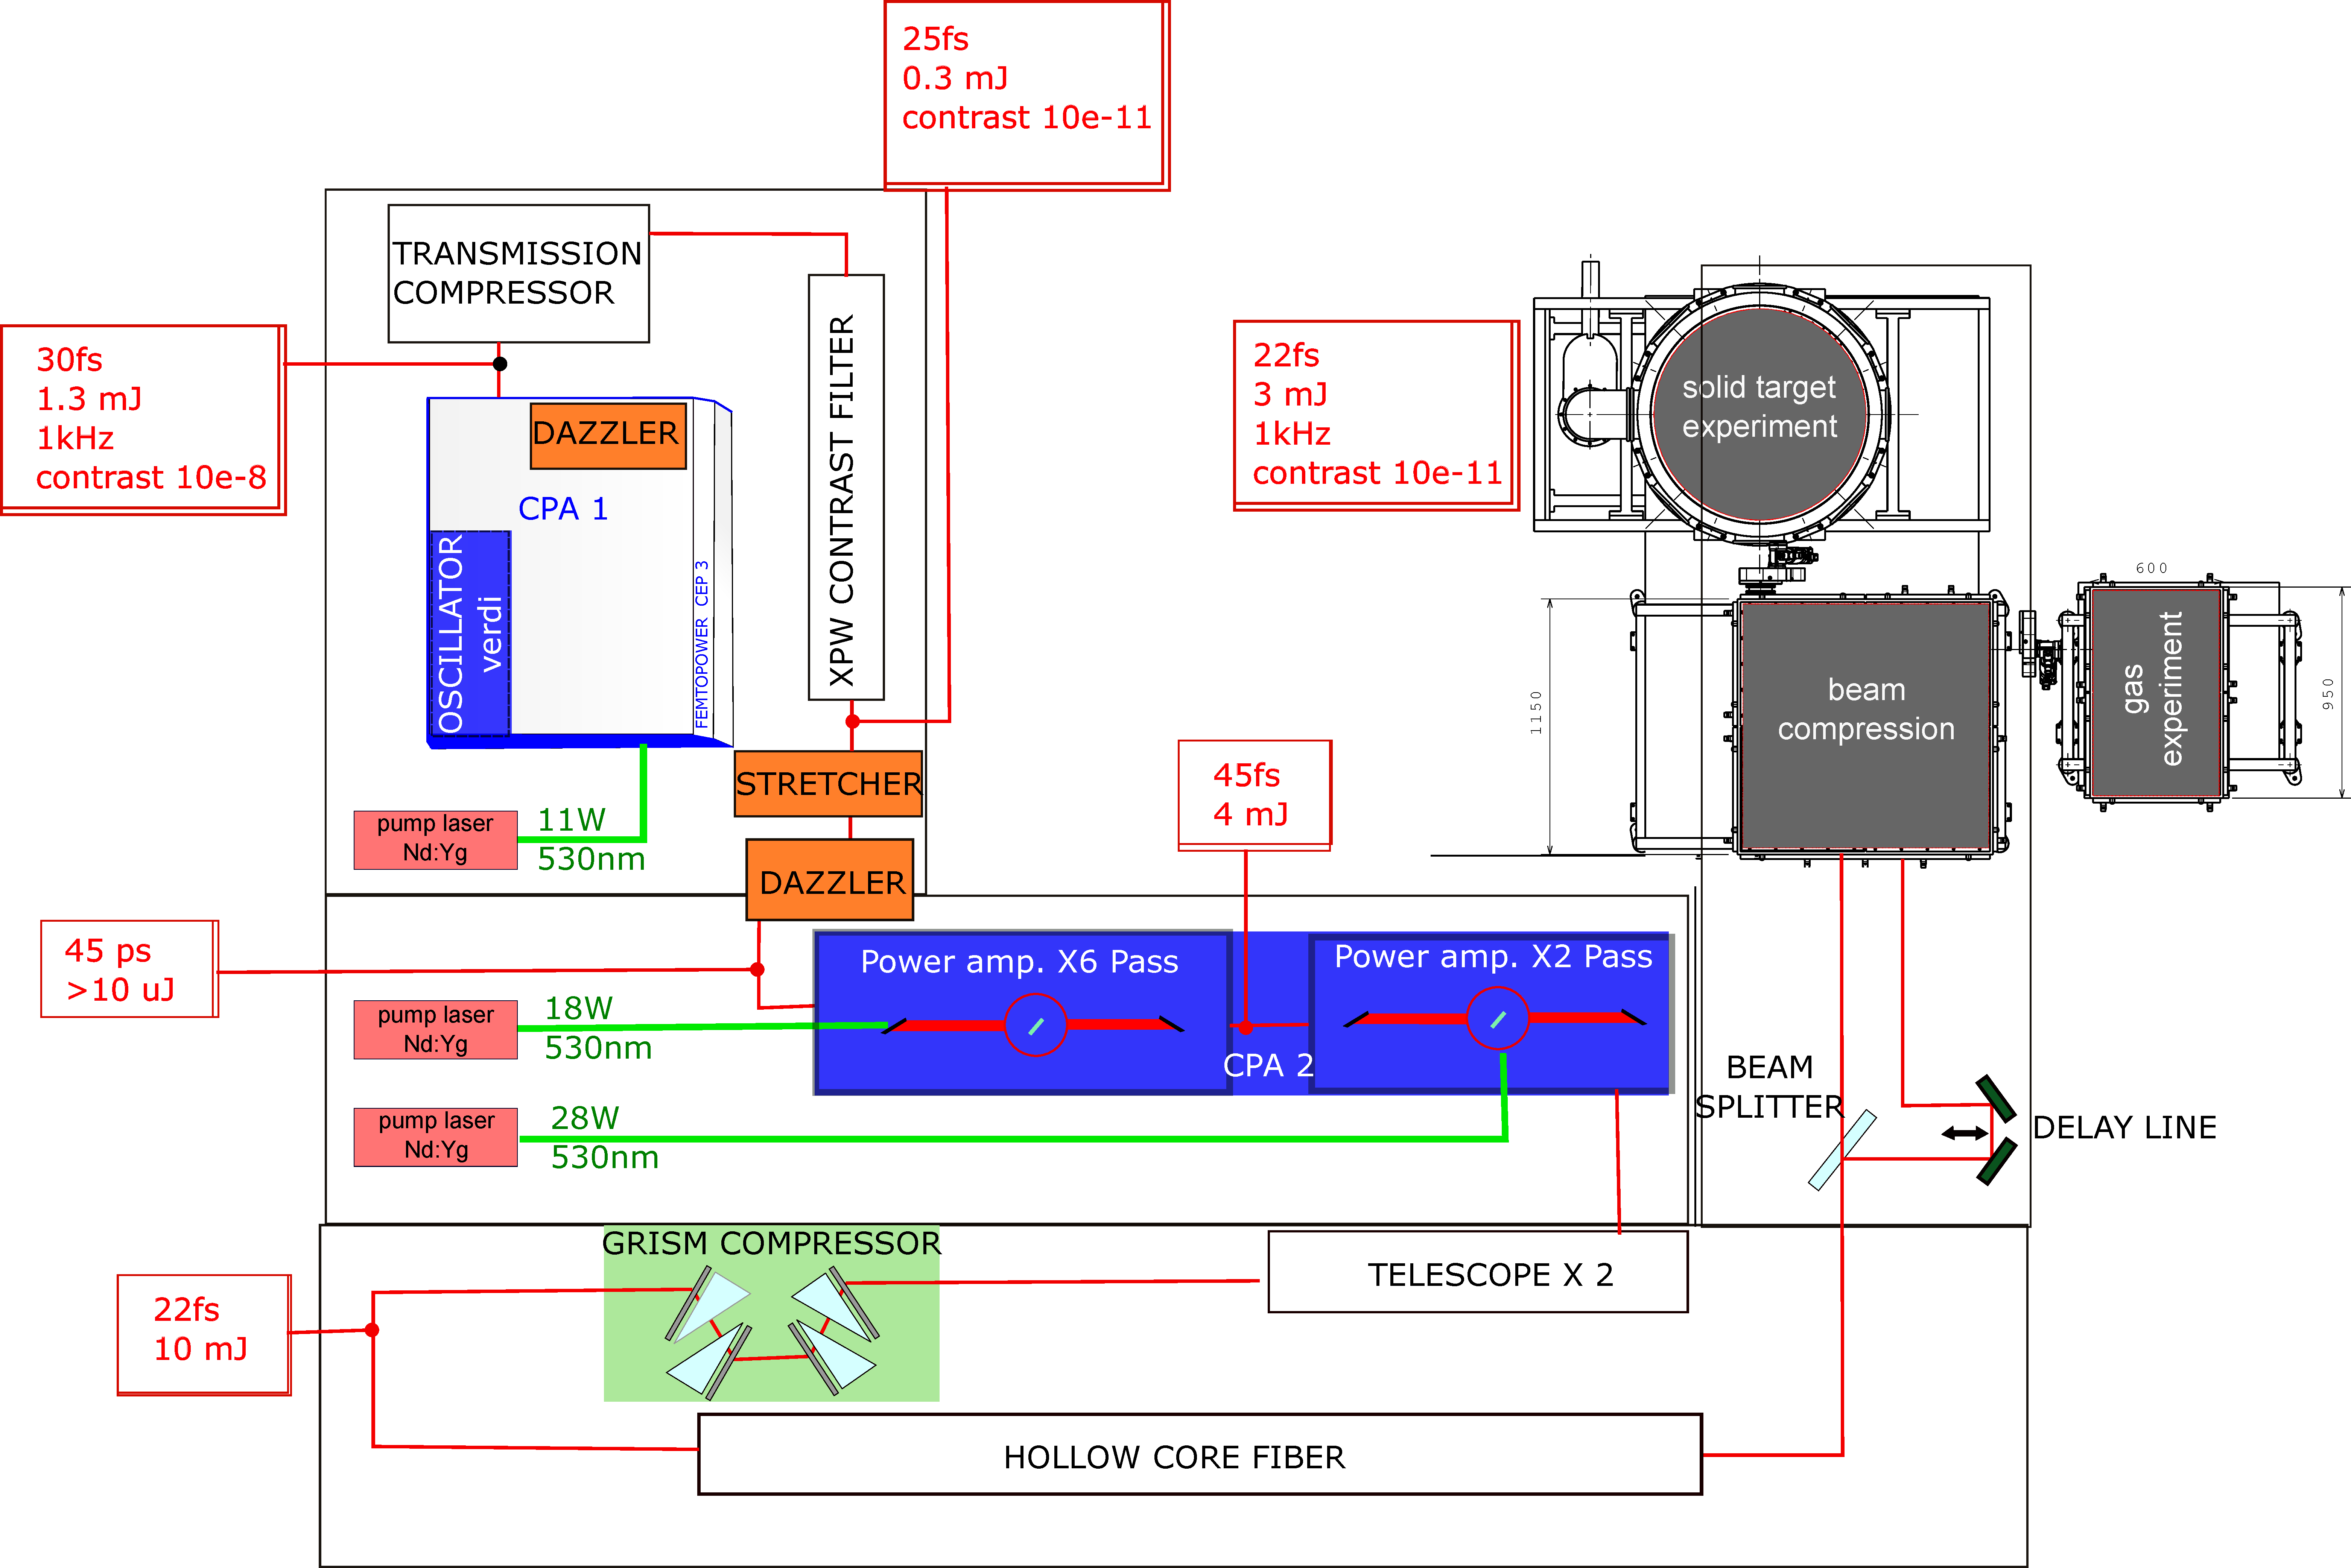
\includegraphics[width =16cm]{../chapitre3/images/femtopower.pdf}\\
\caption{\label{fig:femtopower}Layout of  "Salle Noire" laser}
\end{figure}


%
%
%\subsection{CEP stability of the oscillator}
%
%The oscillator consists of an optical cavity in which is inserted a kerr lens element and delivers in our case a $\sim 7\,\mathrm{fs}$, 2.5nJ pulse train at a repetition of 80 MHz. When the intensity exceeds a given thresold, the kerr lens switches on to the "mode locking mode" (as opposed to "continuous mode"): the oscillator generates a coherent train of femtosecond pulses, or in other word, a frequency comb \cite{holzwarth2000optical,jones2000carrier}.  If every pulse of the train issued by the oscillator were exactly identical, the frequency of the train would rigorously centered on $f_{rep} = 80\,\mathrm{MHz}$ and the resulting spectra would be the superposition of constructing interferences exactely spread by $f_{rep}$ ($\sim 1.7\times 10^{-4}\,\mathrm{nm}$ around 800nm). 
%The Carrier Enveloppe Phase (CEP) is defined by the phase off-set between the maximum of the field intensity and its enveloppe as illustrated in Fig~\ref{fig:TiSa_scheme}. Optical element in the cavity undergo thermal effects and their optical properties can be vary in time which lead the CEP to vary in time. To measure the CEP, the pulse train is sent to a f-2f autocorrelator: each indivdual pulse is duplicated, one of the replica is spectrally broadened and then frequency doubled untill its lowest frequency componants interfere of the highest frequency componants of the first replica.
%It is stabilized by a retroaction of the pump power energy and imposing $f_{ceo} = f_{rep}/4$ (one every forth pulse of the train are identical) with an experimental  rms fluctuation $\sim 360\,\mathrm{mRad}$
%
%The measured spectra is given in Fig\ref{fig:TiSa_scheme}, note that the spectrometer resolution isn't good enough to resolve the spectral beating of the pulse. I practice, CEP fluctuations prevent the train to be rigorously periodic and an unknown beating offset $f_{CEO}$ characterizes the frequency comb.
%
%
%
%\begin{figure}[H]
%\centering
%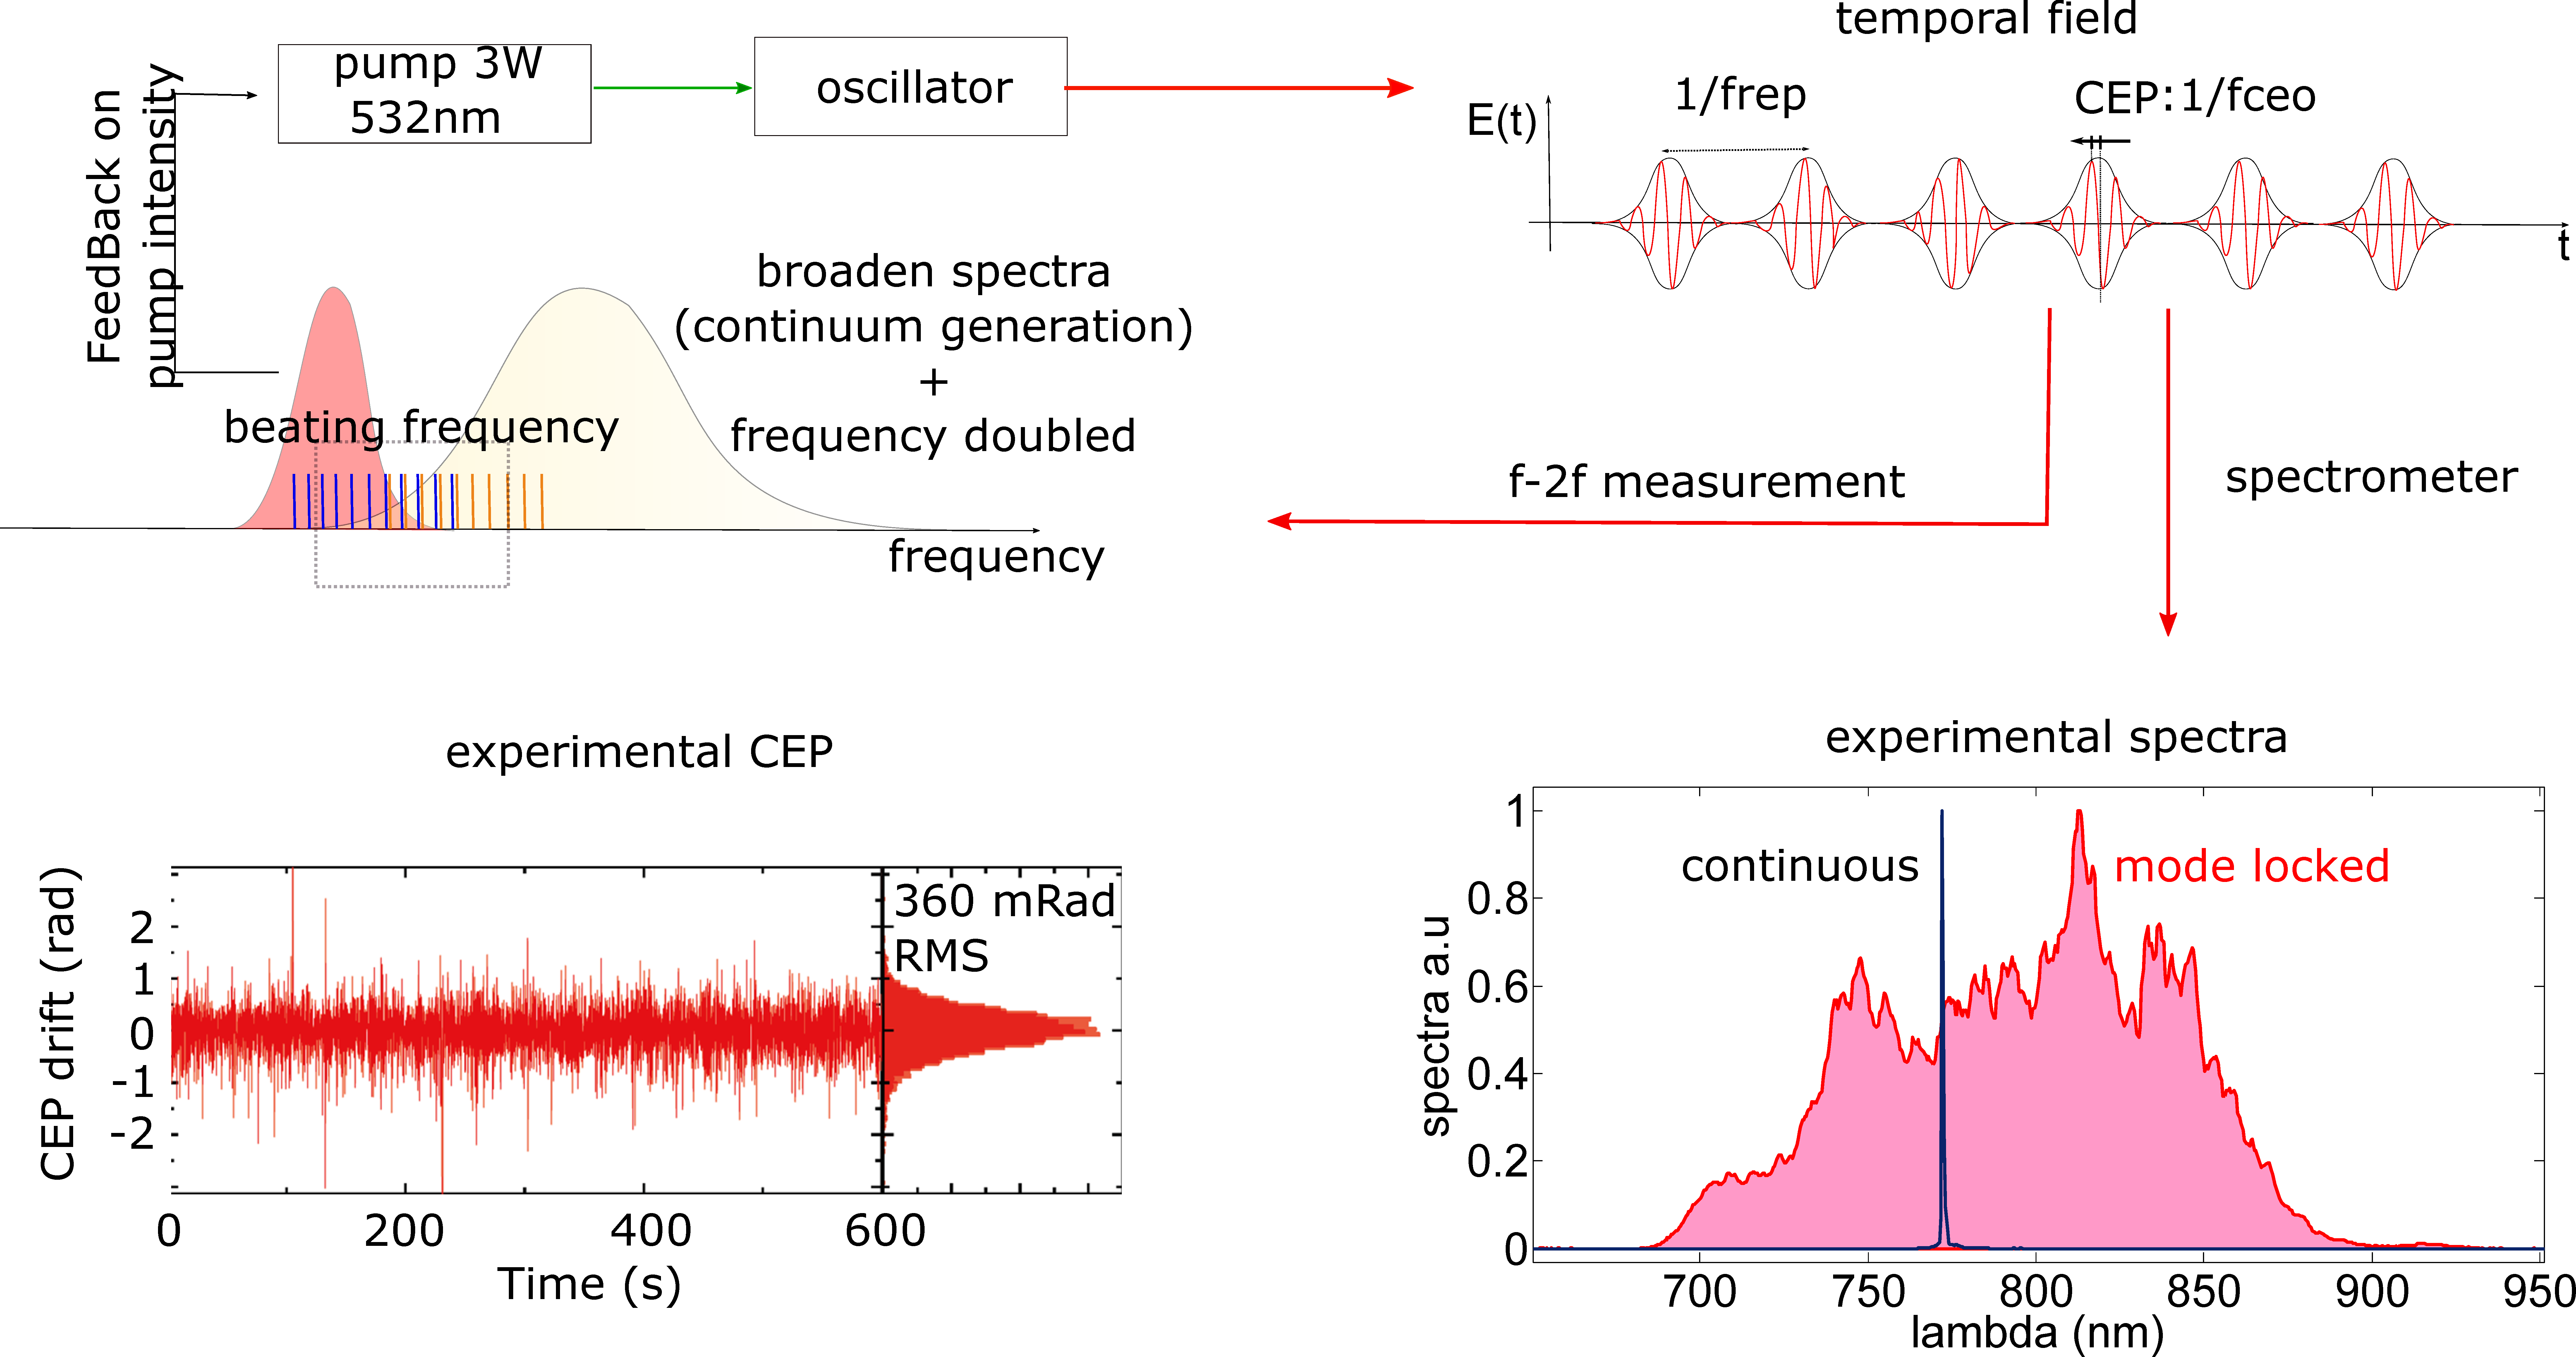
\includegraphics[width =16cm]{../chapitre3/images/TiSa_scheme.pdf}\\
%\caption{\label{fig:TiSa_scheme} CEP stabilization of oscillator}
%\end{figure}
%
%
%
\subsection{XPW contrast cleaning}
\label{subsection:XPW contrast cleaning}

The temporal contrast of a laser pulse is defined by the ratio of the intensity at time~$t$ and the maximum intensity measured on long time scales with respect to the pulse duration (picosecond to nanosecond). It is a critical parameter in laser-solid plasma interactions since it determines the actual interaction conditions of the laser peak intensity with the plasma. Indeed, as we already discussed in the introduction, a portion of the pulse energy is contained in the temporal pedestal picoseconds to nanoseconds. This pedestal is mainly constituted by a nanosecond-long pulse resulting from ASE\footnote{Amplified Spontaneous Emission}, intense enough to preionize a dielectric target for intensities $\sim 10^{10-11}\mathrm{W/cm^2}$~\cite{bloembergen1970fundamentals,stuart1995laser} and prepulses which sub-picosecond durations where the ionization threshold intensities are typically $\sim 10^{13-14}\mathrm{W/cm^2}$~\cite{gamaly2002ablation}. The plasma therefore has time to expand before the interaction with the pulse peak and dramatically change the non-linearity of the interaction (HHG generation collapses with long plasma scale length as indicated in~\ref{subsection:Collective response of density gradient}\label{subsubsection:Collective response of density gradient}). To increase the contrast, different techniques have been implemented: saturable absorbers, electro-optic switches up to a few ns before the main pulse \cite{nantel1998temporal}, non-linear rotation of polarization \cite{homoelle2002pulse,tapie1992shaping}, plasma mirrors \cite{doumy2004complete,kapteyn1991prepulse,ziener2003specular}. In our laser chain, we use a XPW (Cross-Polarized four Wave mixing process)\cite{jullien200510} to increase the contrast after the first CPA, as represented in Fig~\ref{fig:TiSa_scheme}: the S polarized (with respect to the Glan polarizer) femtosecond output propagates non-linearly ($\chi^{(3)}$) in BaF$_2$ crystals after going through a hollow core fiber for spatial filtering, and coherently generates a cross polarized beam (called XPW) with an efficiency proportional to $(I/I_{max})^3$. The XPW pulse has an improved contrast and is selected with a Glan polarizer. Because the overall efficiency of the process is $\sim 25\%$, two additional Ti:Sa amplifiers, represented on Fig~\ref{fig:femtopower}, are necessary to increase the laser energy to more than $10$mJ. \\



\begin{figure}[H]
\centering
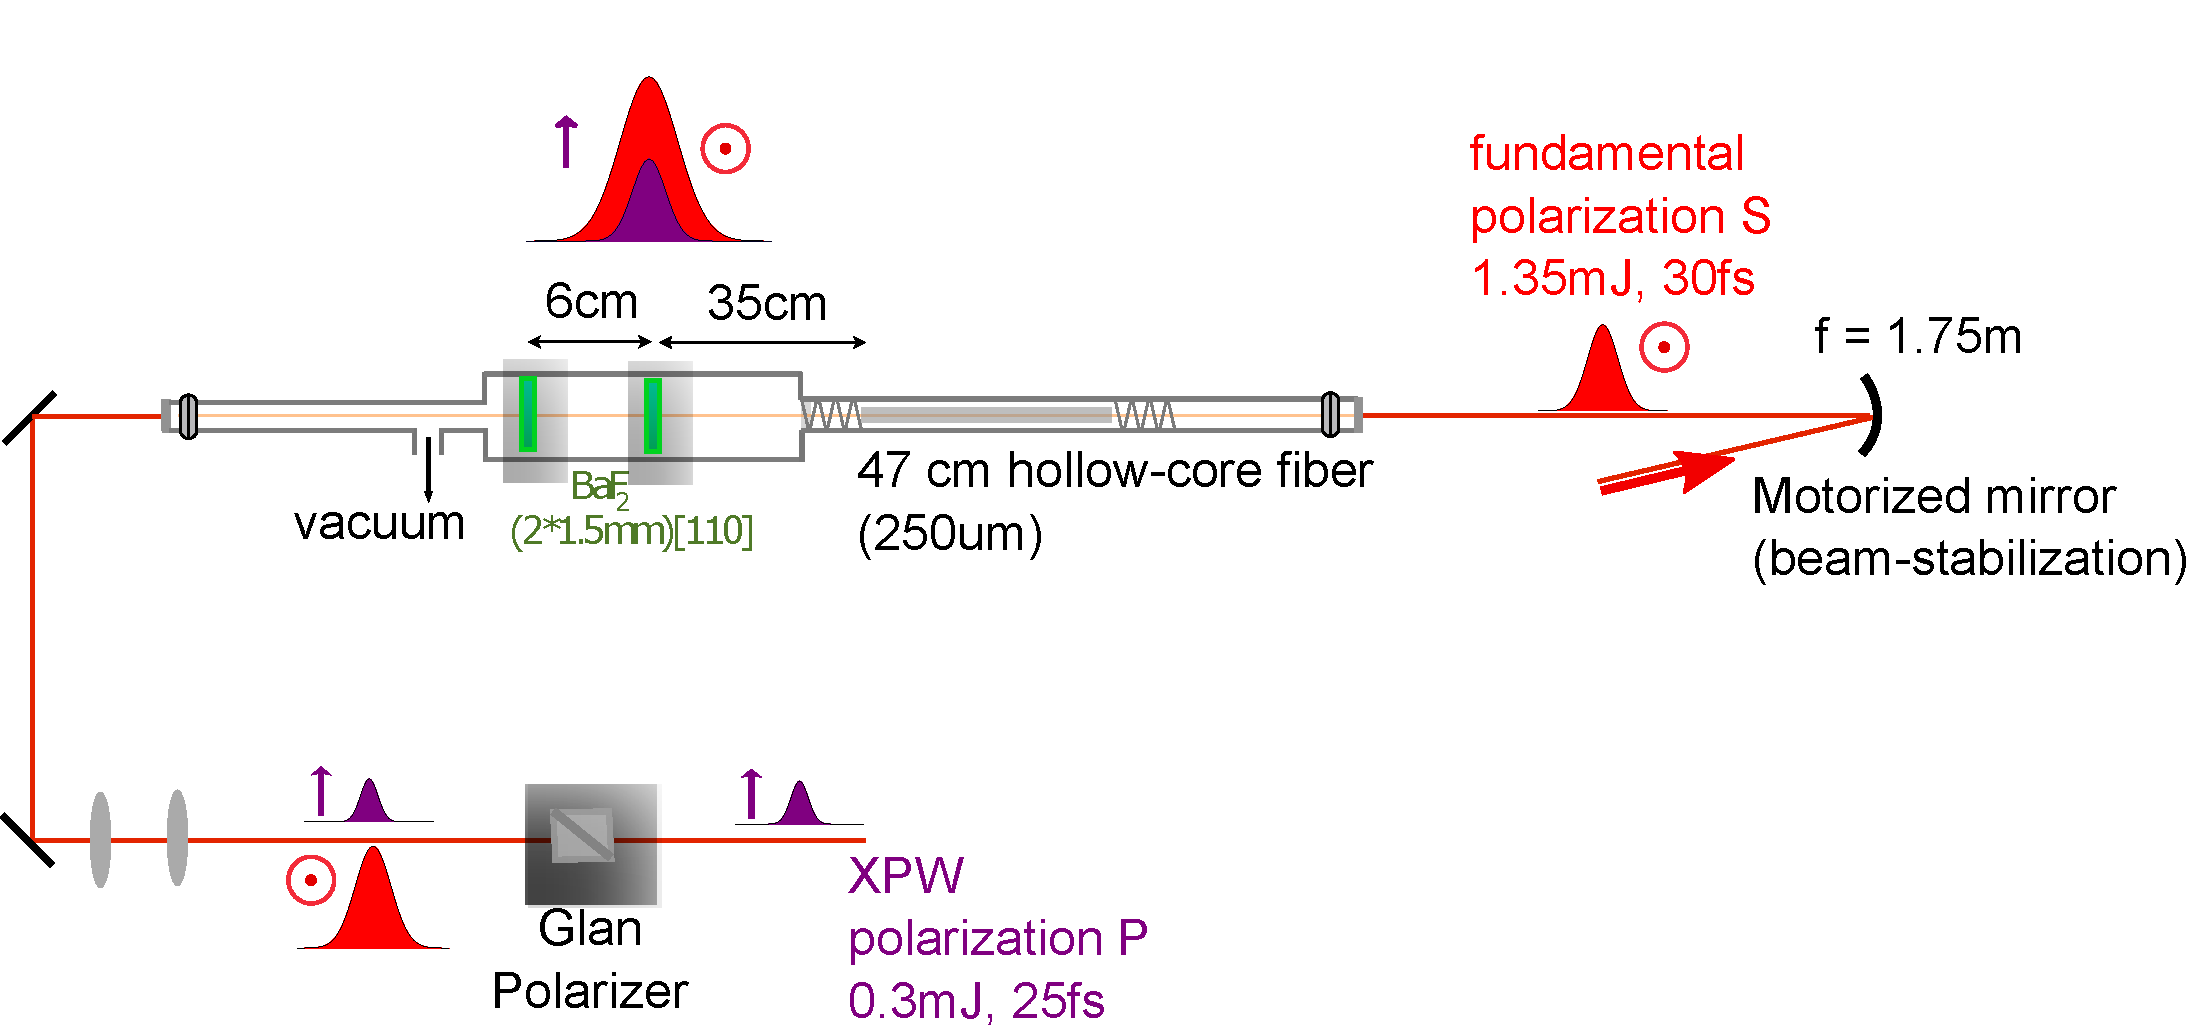
\includegraphics[width =16cm]{../chapitre3/images/XPW.pdf}\\
\caption{\label{fig:TiSa_scheme} Principle of XPW (Cross Polarization Wave mixing): a S polarized 30fs pulse propagates non-linearly ($\chi^{(3)}$  ) in BaF$_2$ crystals and coherently generates a crossed polarized beam (called XPW) with an efficiency proportional to $(I/I_{max})^3$. The XPW pulse has an improved contrast and is selected with a Glan polarizer}
\end{figure}

\noindent We performed a contrast measurement using a commercial third-order autocorrelator (Sequoia, from \textit{Amplitude Technologies}). The compressed pulse is split into two replicas. One replica is frequency doubled in a SHG crystal and later combined, at a given delay, with the second initial replica to generate the third harmonic of the initial pulse. The resulting signal is detected with a photomultiplier and reaches its maximum when the pulses overlap, that is to say at $t=0$. 

\begin{figure}[H]
\centering
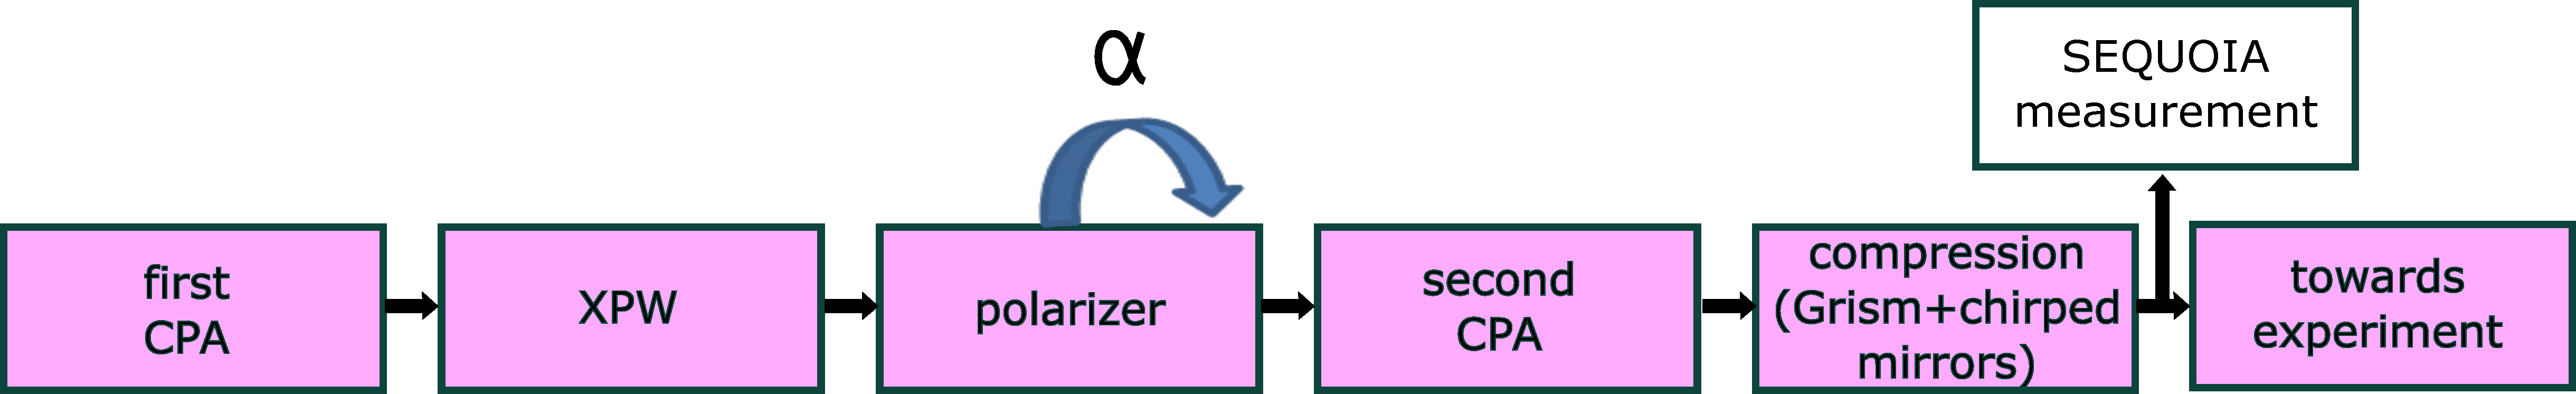
\includegraphics[width =15cm]{../chapitre3/images/XPW-sceme.pdf}\\
\caption{\label{fig:XPW-sceme} Contrast measurement after XPW contrast cleaning. $\alpha$ is the polarizer angle. $\alpha =0$ corresponds to optimal alignment.}
\end{figure}

\begin{figure}[H]
\centering
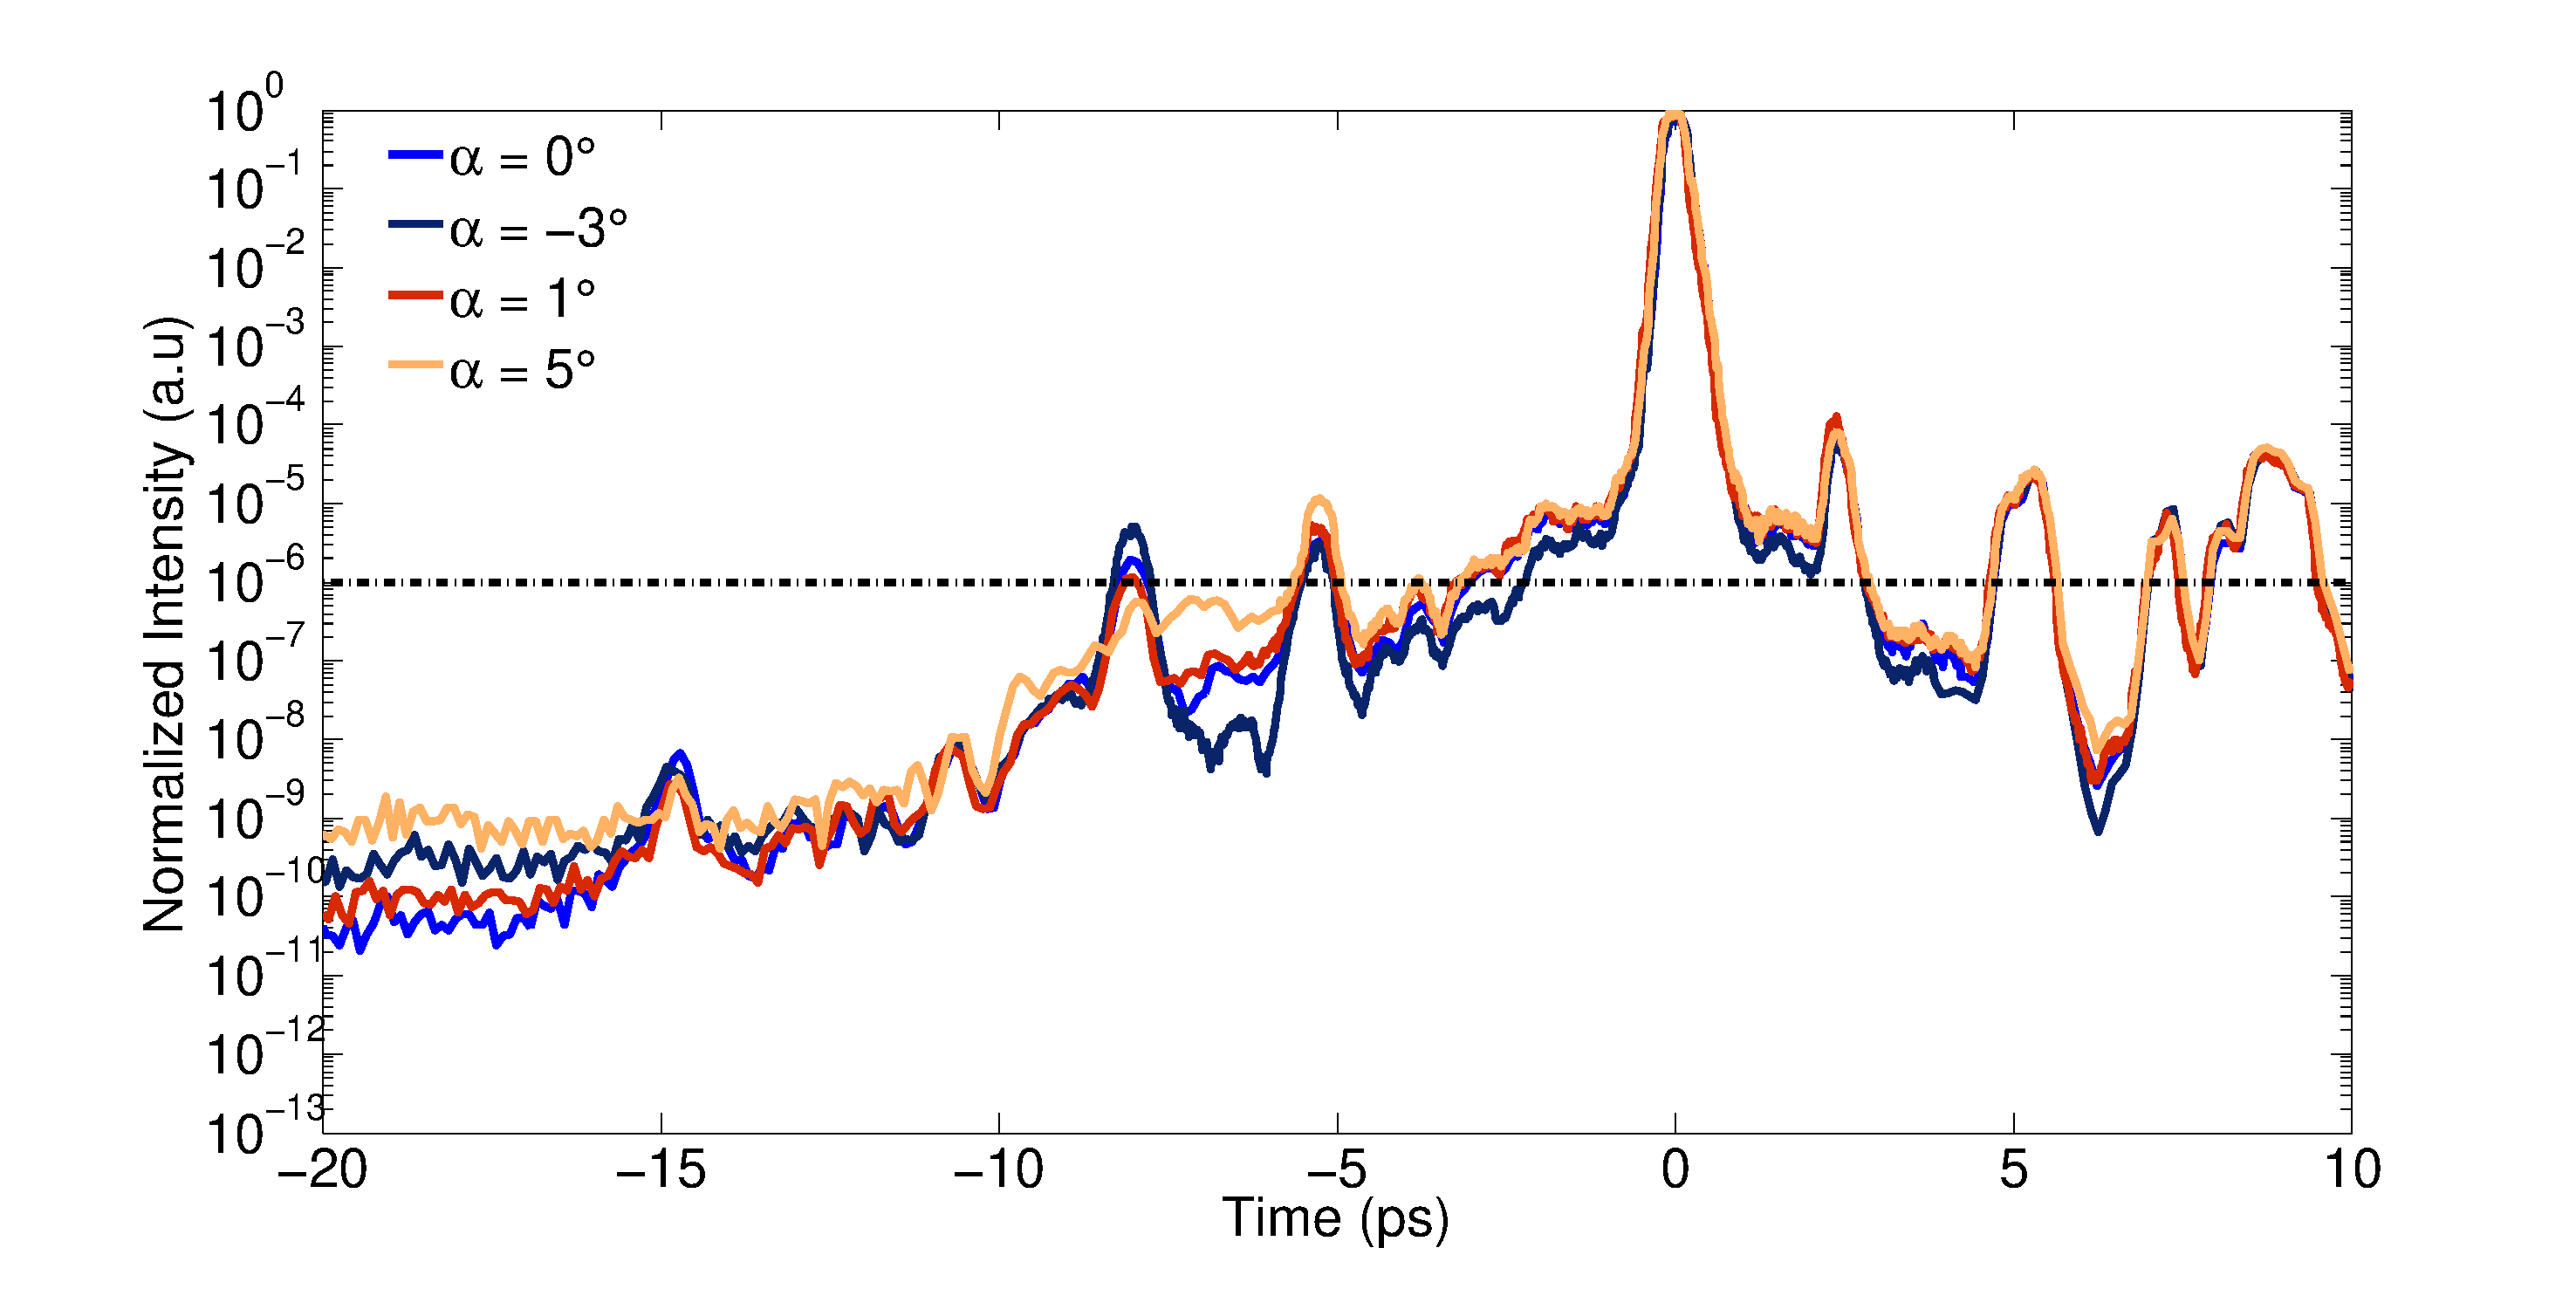
\includegraphics[width =15cm]{../chapitre3/images/EffectContrast_XPWangle.pdf}\\
\caption{\label{fig:EffectContrast_XPWangle2} SEQUOIA contrast measurement for different angles of the polarizer after XPW. The dotted horizontal line represents an ionization threshold for fused silica arbitrarily set to $10^{12}\,\mathrm{W/cm^2}$ as an indicator (for $I_{max} = 10^{18}\,\mathrm{W/cm^2}$)}
\end{figure}



 \noindent On the contrast measurement shown in Fig~\ref{fig:EffectContrast_XPWangle2}, we can appreciate the effect of the polarizer angle on the contrast measured after the double CPA followed by compression. The best contrast is obtained for $\alpha = 0^{\circ}$ on the long temporal range (up to nanoseconds, not represented here) and reaches $10^{-11}$ at -$20\,\mathrm{ps}$ before the arrival of the main pulse. However, around $-8\,\mathrm{ps}$, the contrast is on the contrary improved for a polarizer $\alpha = 5^{\circ}$, and around $-5\,\mathrm{ps}$, for $\alpha = -3^{\circ}$. This observation has its importance and introduces what we call coherent contrast : when the laser is filtered by the XPW, the higher orders of the spectral phase induce temporal fluctuations which can extend up to $\sim 20\,\mathrm{ps}$ before and after the main pulse. The laser pulse goes into the 2$^{nd}$ CPA where nonlinearities induce phase modulations, and therefore modulation of the coherent contrast. This is very sensitive to a fine alignment of the XPW, and the optimal angle to filter out the long temporal range contrast is not necessarily the same for the coherent, ie short dynamic range contrast. As a consequence, the coherent contrast (t>-20ps typically) can be degraded and prepulses with intensities high enough to preionise the target can emerge. 

\subsection{Spectral clipping}
\label{subsection:Spectral clipping}

Any amplitude modulation, such as spectral clipping on the optics, leads to coherent contrast degradation. This spectral clipping can be prevented by narrowing  the pulse spectrum (using the Dazzler). The cost associated with this apodization is an increased duration of the compressed pulse. 
In Fig~\ref{fig:EffectContrast_XPWangle}(a), we measured the contrast between -100ps and 10ps. The dotted line at -20ps arbitrarily separated the incoherent contrast ($10^{-11}$ for t < -20ps) from the coherent contrast ( t >-20ps ). In Fig~\ref{fig:EffectContrast_XPWangle}(b) we simply zoomed on the coherent contrast and we can clearly see the degradation (prepulse at -3ps) due to spectral clipping.



\begin{figure}[H]
\centering
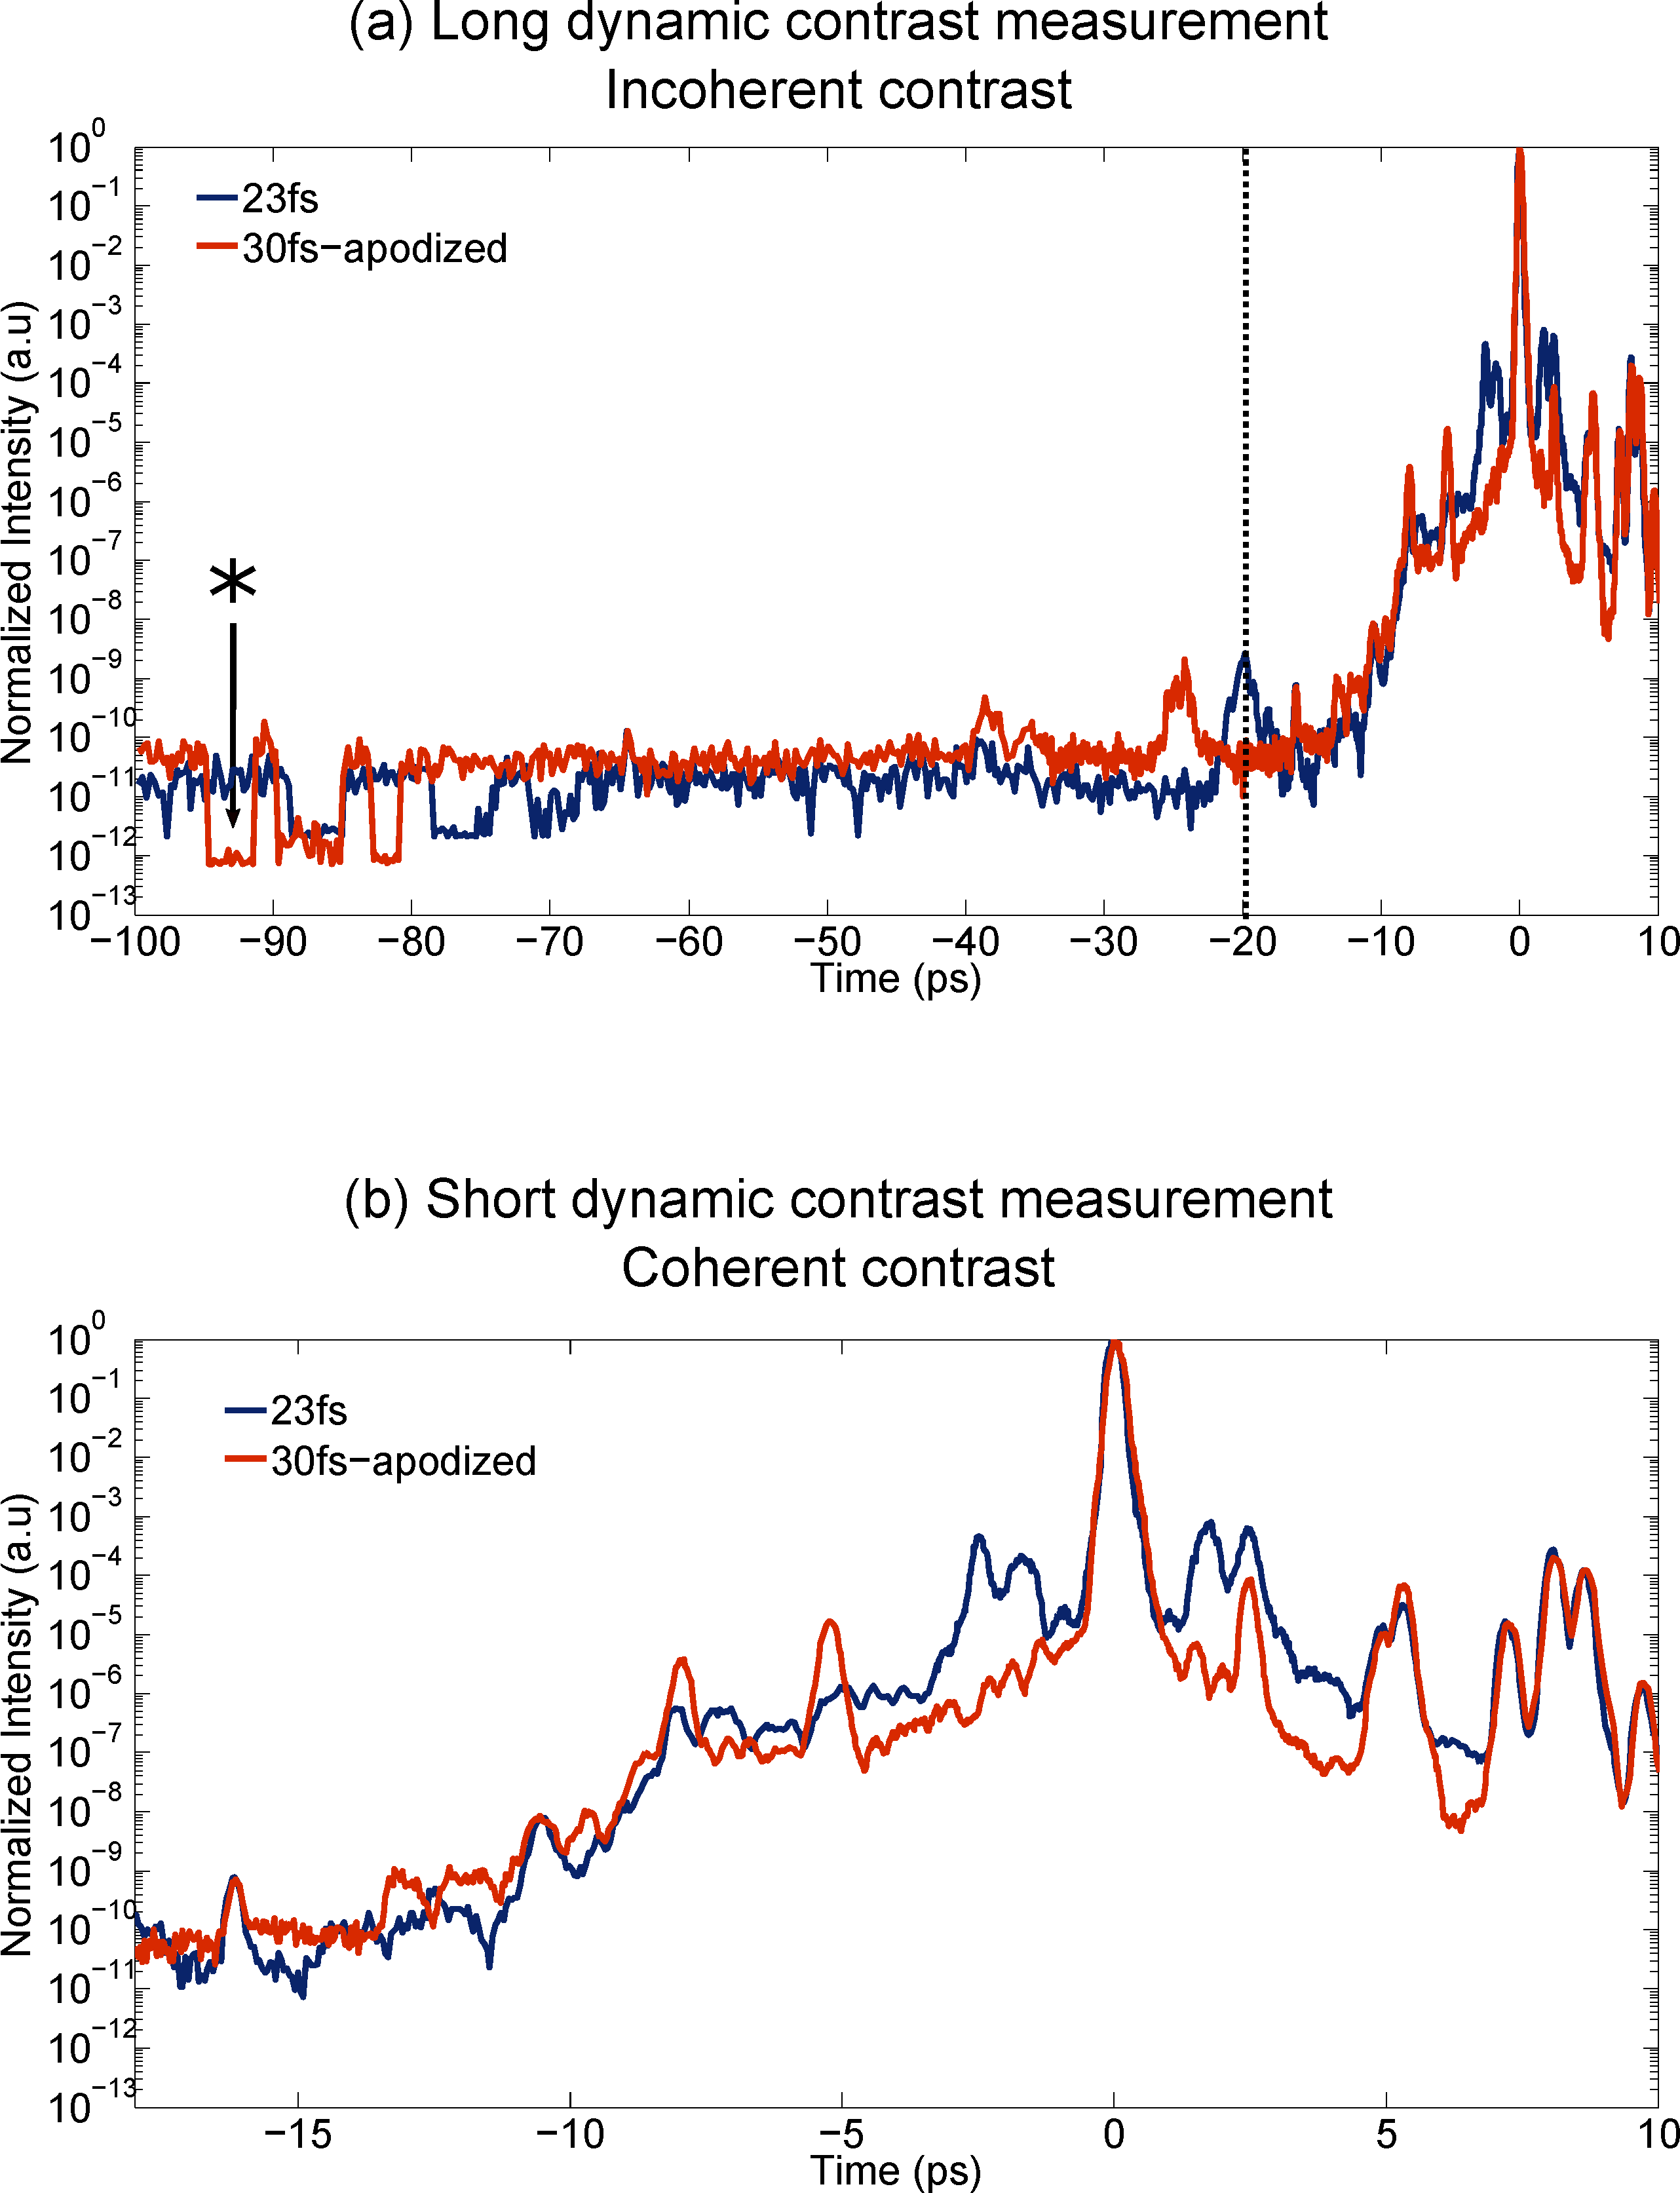
\includegraphics[width =10cm]{../chapitre3/images/Apodized_vs_NonApodized.pdf}\\
\caption{\label{fig:EffectContrast_XPWangle} SEQUOIA contrast measurement using sequoia after the double CPA with or without is apodization by the dazzler (respectively 30fs and 23fs FTL). (*) beam is blocked to show detector noise level}
\end{figure}

\subsection{Prepulse generation from post-pulses}

We have identified an important source of degradation of the laser contrast: post-pulses. In theory, post-pulses arrive by definition after the main pulse, so they cannot contribute to the target degradation prior to the interaction. However, a non-intuitive phenomenon occurs when a post-pulse propagates nonlinearly in a CPA (high B integral) after the beam has been stretched: a prepulse is generated. This problem has already been described in the context of CPA amplification \cite{oakley1998improving,ren2010pulse,bromage2012temporal} and has been verified experimentally \cite{oakley1998improving,didenko2008contrast}. We show here, as suggested in~\cite{kalashnikov2009limits}, that nonlinear effects in CPA materials where the B integral is large are responsible for contrast degradation and can generate prepulses.\\



\noindent The experimental demonstration of this effect is summarized in~Fig~\ref{fig:WindowsContrastDegradation-2} where two optical elements (output window of XPW setup, beam splitter for diagnostics prior to amplification) are removed one after the other. We clearly see on the contrast measurement the successive suppression of the prepulses at respectively $-8$ps and -$6$ps. \\



\begin{figure}[H]
\centering
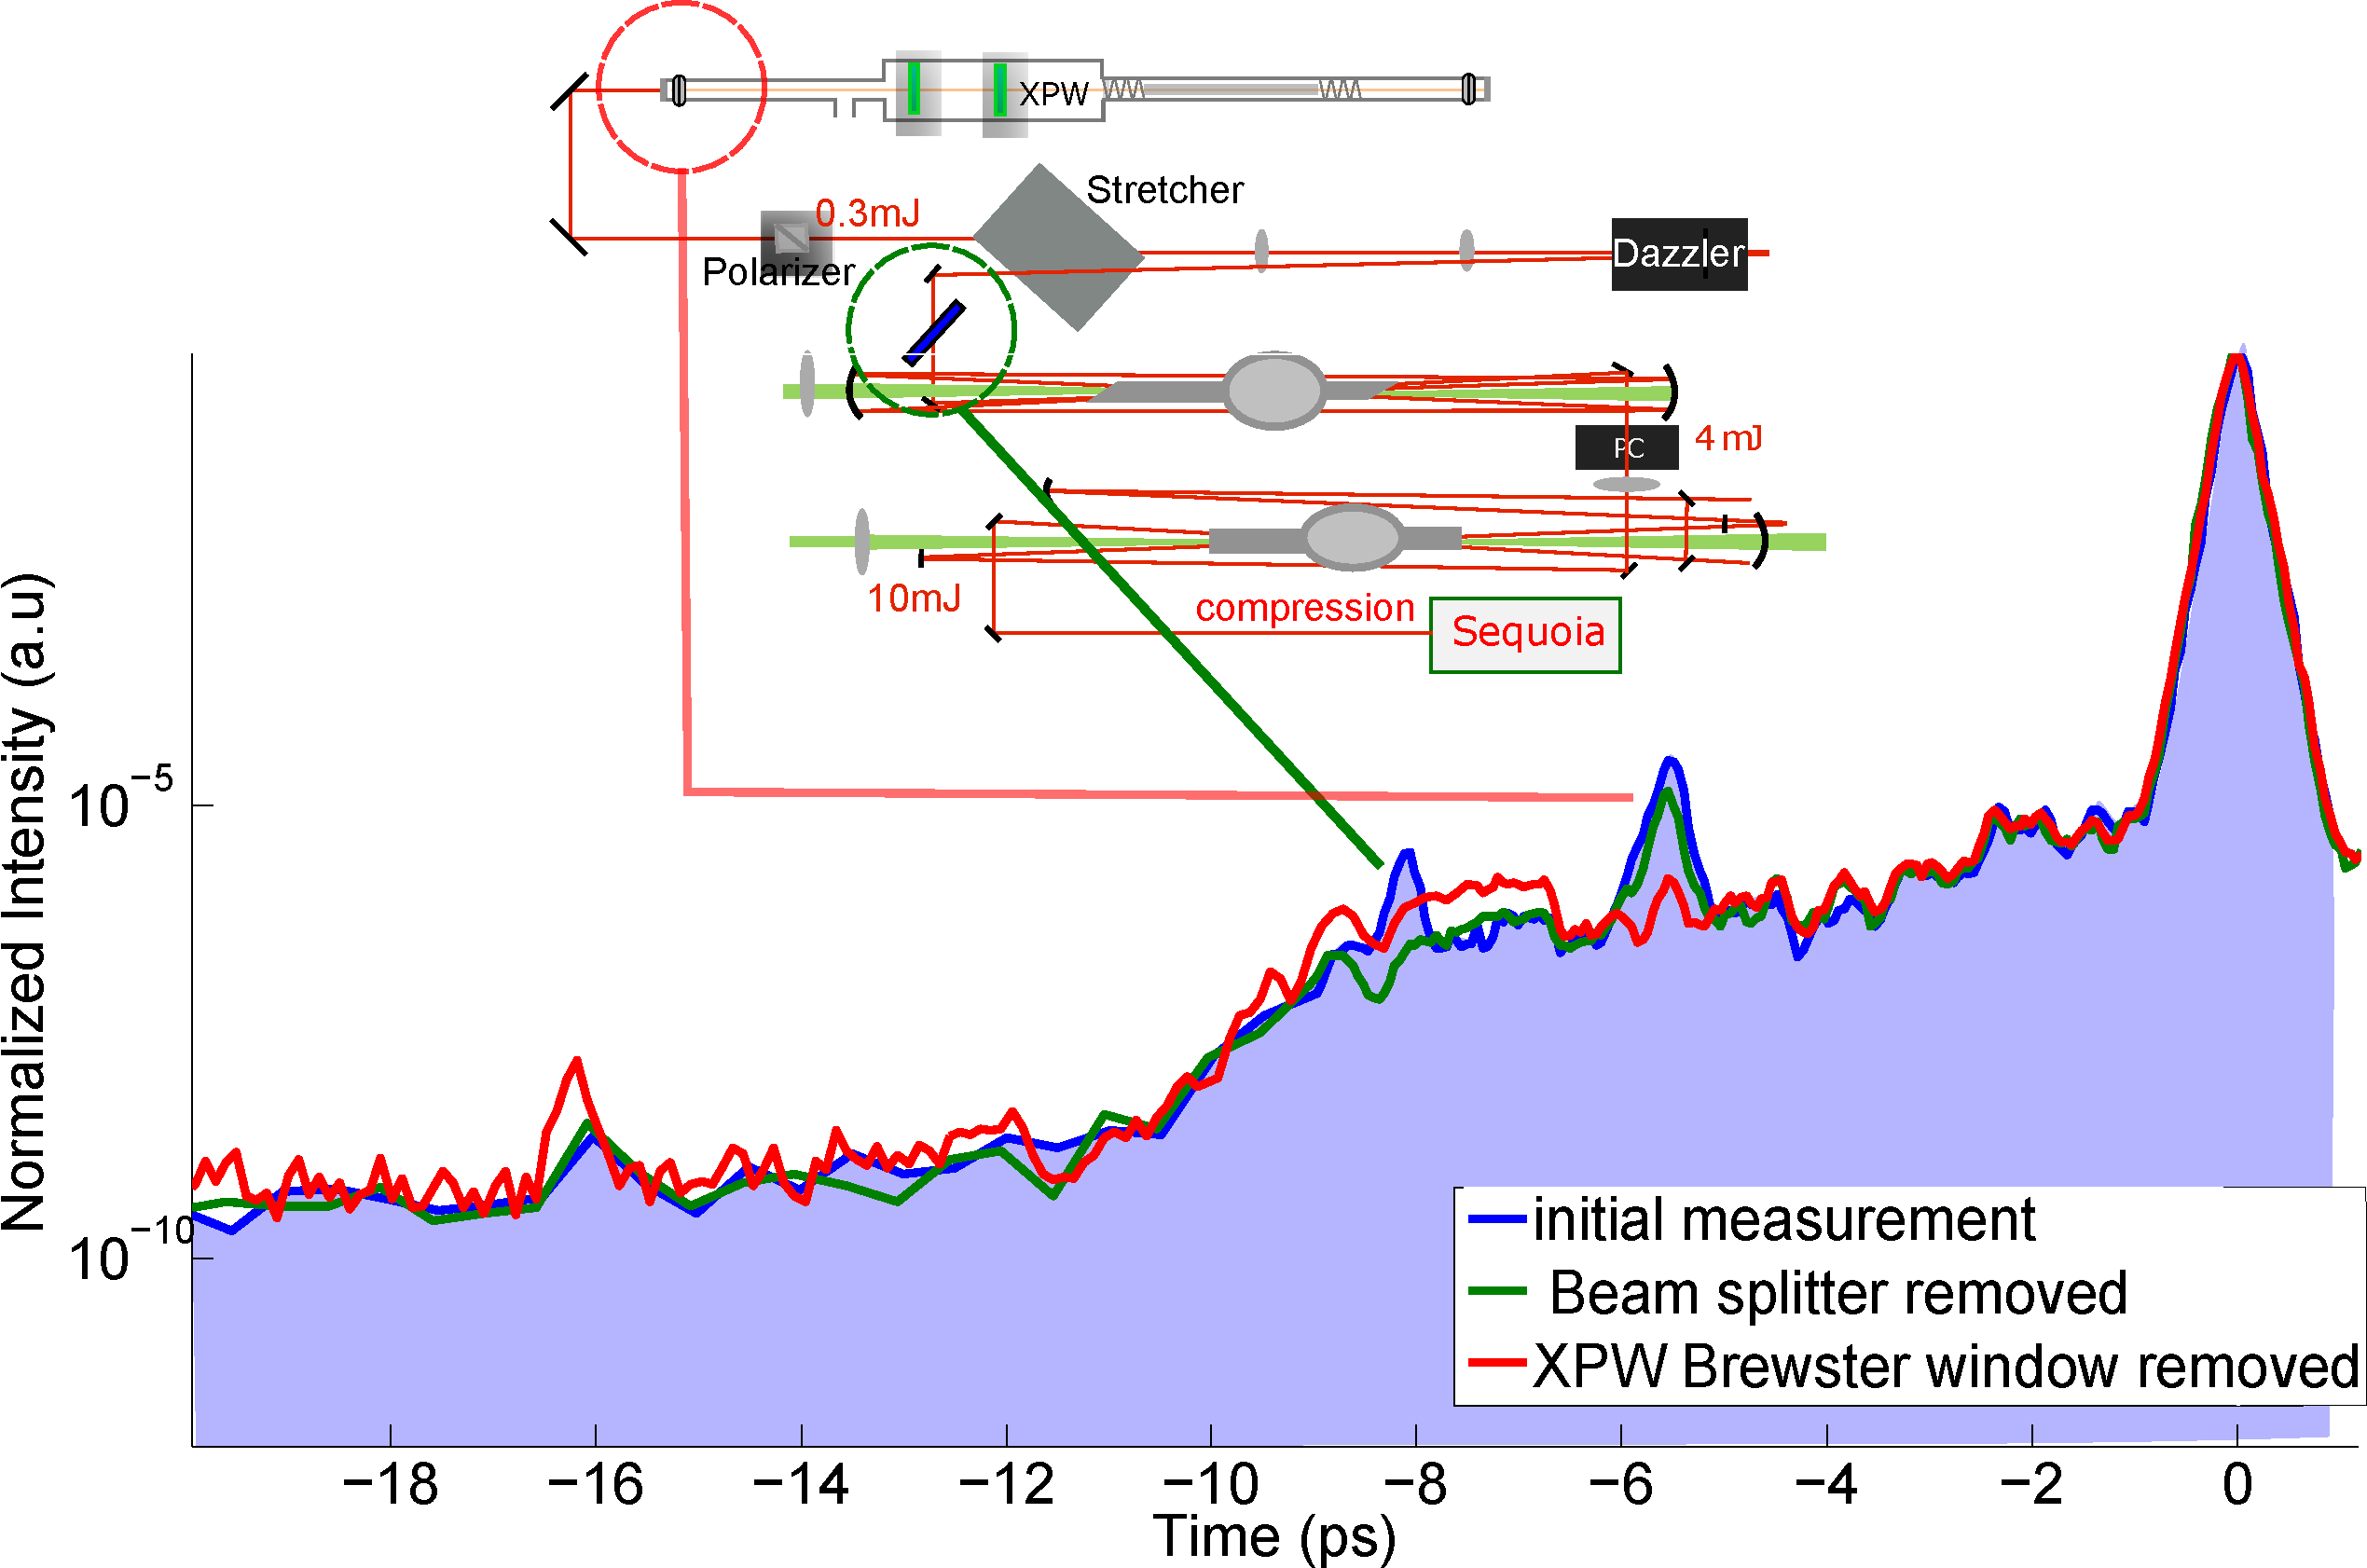
\includegraphics[width =16cm]{../chapitre3/images/WindowsContrastDegradation-3.pdf}\\
\caption{\label{fig:WindowsContrastDegradation-2} Comparative temporal contrast measurement: removal of optics prior to the second CPA which induce post-pulses, and hence prepulses after the second CPA}
\end{figure}

\noindent We now show how self-phase modulation (SPM) can account for this behavior. We do not take into account the spatial profile of the pulse as it does not help to highlight the 
physical origin of nonlinear prepulse generation. We consider a laser pulse of duration $\sigma_t$ in Fourier limit, defined by its temporal variable only. We model the effect of an arbitrary stretcher using analytical relations found in~\cite{TheseArnaud}, and we add an identical postpulse of relative amplitude $\eta$ at a delay $\tau$:

\begin{equation}
\label{eq:fieldDef}
E(t) = A_{0}(t)\exp(-i\omega_0 t)+\eta A_0(t-\tau)\exp(-i\omega_0 (t-\tau))
\end{equation}

\noindent where the temporal envelop $A_0$ is defined by~\cite{TheseArnaud}:

\begin{equation}
\label{eq:tempEnv}
A_0(t) = \exp(-\frac{t^2}{2(1+\xi^2)\sigma_t^2})\exp(-i\phi(t))
\end{equation}


\noindent  where $\xi = \frac{\phi^{(2)}}{\tau_t^2}$ is the normalized spectral chirp induced by the stretcher and: 
$$
\phi(t) = \frac{1}{2\sigma_t^2}\frac{\xi t^2}{1+\xi^2}+ \frac{1}{2}\arctan(\xi)
$$

\begin{figure}[H]
\centering

\includegraphics[width =\textwidth]{../chapitre3/images/ModelizeingSPM.pdf}\\
\caption{\label{fig:ModelizeingSPM} Block diagram describing the operations performed on the initial pulse leading to prepulse generation. The first three blocks are contained in Eq~\ref{eq:fieldDef} and Eq~\ref{eq:tempEnv}. The pulse is compressed by imposing a negative chirp opposite to that induced by the stretcher.}
\end{figure}

\noindent  Since the effect we want to illustrate is due to the nonlinear index of the material, the simplest approach is to consider \g{Self-Phase-Modulation}, which is the "first order" temporal nonlinearity to consider in a material.
If we neglect dispersion and spatio-temporal couplings, and in the slowly varying envelope approximation, the accumulated nonlinear temporal phase is given by:

\begin{equation}
\phi_{NL}(t) = \gamma|E(t)|^2
\end{equation}

\noindent  Where $\gamma = \frac{n_2\pi}{\lambda}$ which gives, after development using~\ref{eq:fieldDef}:

\begin{equation}
\label{eq:Interf}
\phi_{NL}(t) = \gamma|A_0(t)|^2+\gamma\eta^2|A_0(t-\tau)|^2+2|A_0(t)A_0(t-\tau)|\cos(\phi(t)-\phi(t-\tau)+\omega_0\tau)
\end{equation}

\noindent In addition, \g{the B integral} is a measure of the amount of non-linear phase accumulated induced by propagation of a pulse of intensity I over a distance $L$ inside a material defined by its non-linear index $n_2$, and is expressed by the relation:

\begin{equation}
B[\,\mathrm{Rad}] = \frac{2\pi}{\lambda}L \int_{0}^{L}n_2 I(0,z)dz
\end{equation}
\noindent  When the two stretched pulses do not overlap, we have by definition $A_0(t)A_0(t-\tau) = 0$ which cancels the interference term in Eq~\ref{eq:Interf}. When they overlap, the temporal phase oscillates in the overlapping region. When the pulse is positively chirped, the blue frequencies are delayed relative to the red ones, therefore the blue will be modulated in case $\xi>0$. When the pulse is negatively chirped ($\xi < 0$), it is the opposite and the red component will overlap with the postpulse, and therefore be modulated. This is illustrated in Fig~\ref{fig:SpectralBeating} where we show the spectrum of the pulse when we add SPM on the stretched pulse for $\xi = 5$ and $\xi = -5$, after recompression.


\begin{figure}[H]
\centering
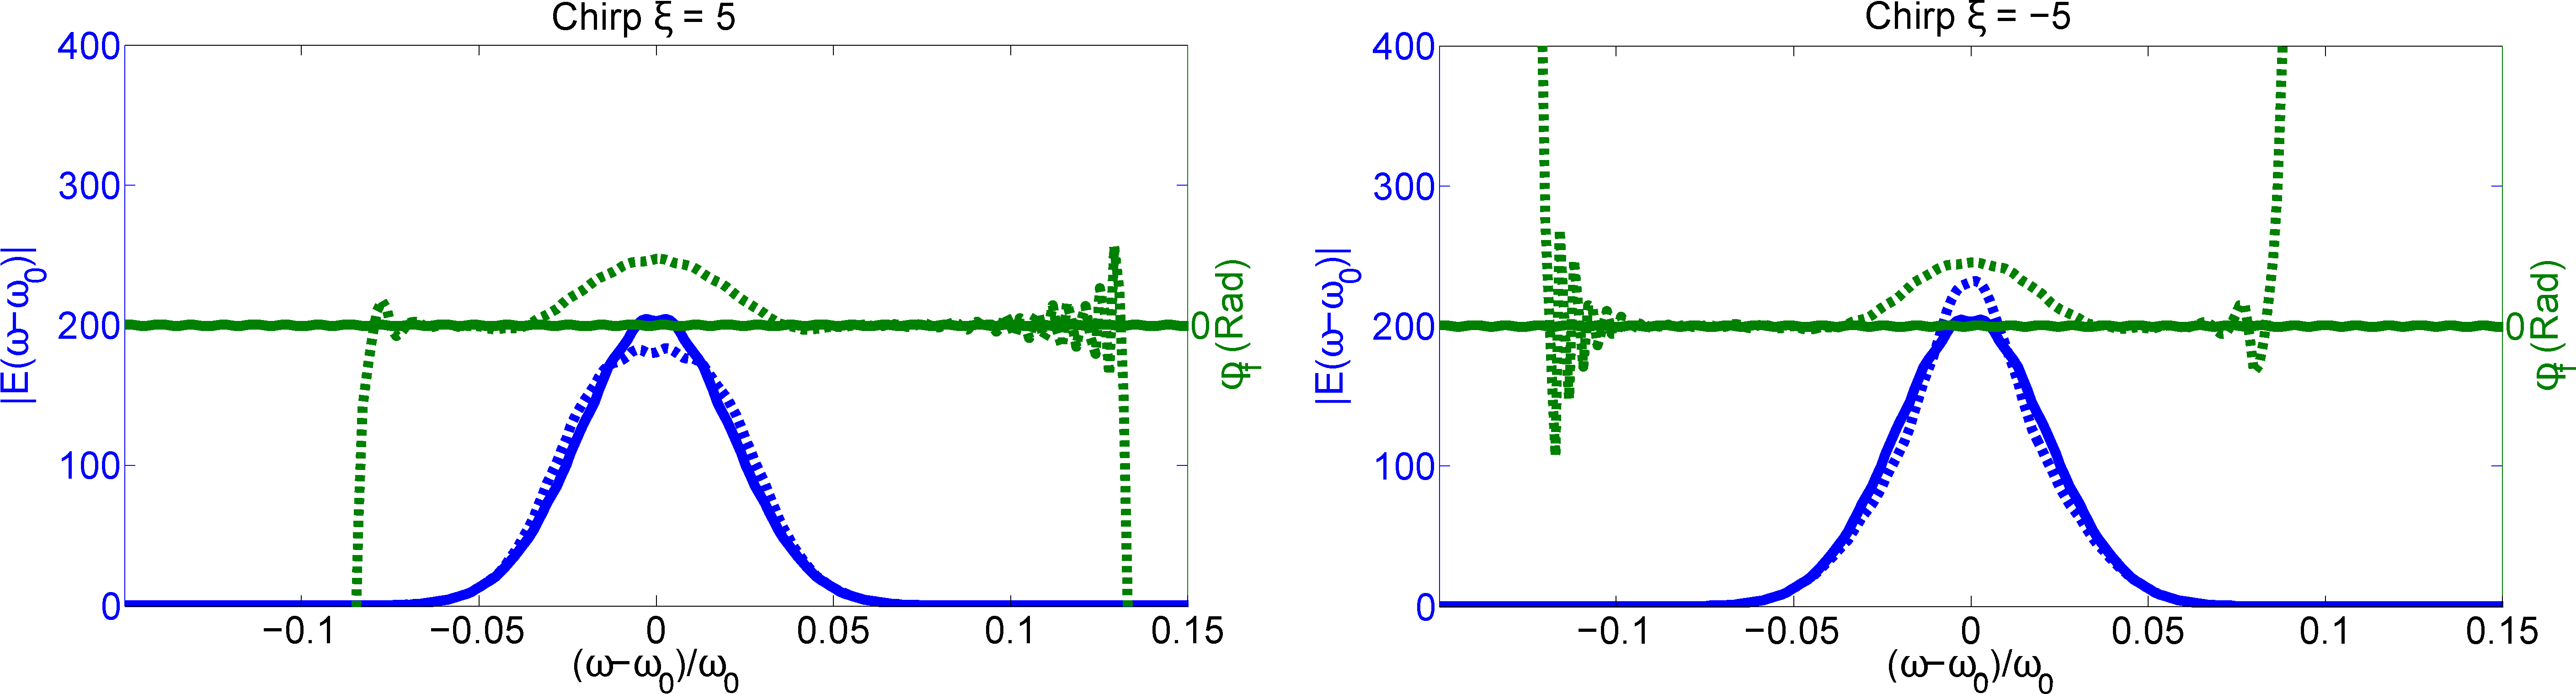
\includegraphics[width =\textwidth]{../chapitre3/images/SpectralBeating.pdf}\\
\caption{\label{fig:SpectralBeating} Spectrum and phase prior to pulse stretching (continuous lines) and after compression (dotted lines) with a postpulse of $\eta = 1\%$ relative intensity added prior to stretching. The chirp factor introduced by the stretching is $\xi = \pm 5$. When $\xi>+5$ (left), higher phase modulations appear in the blue part of the spectrum. When $\xi <-5$ (right) higher phase modulations appear in the red part of the spectrum.}
\end{figure}




\noindent  The high-order phase modulations described above can of course only occur when the main pulse overlaps with its delayed replica. In Fig~\ref{fig:Result_NL=1}, we vary the stretching factor from $\xi = 0$ (no stretching) to $\xi = 5$. The initial temporal profile of the pulse is represented on a linear scale on the left column for each $\xi$, and the corresponding temporal profiles after stretching+SPM+compression in logarithmic scale on the right column: for $\xi = 5$, a prepulse with relative intensity $> 10^{-4}$ is clearly visible.

\begin{figure}[H]
\centering
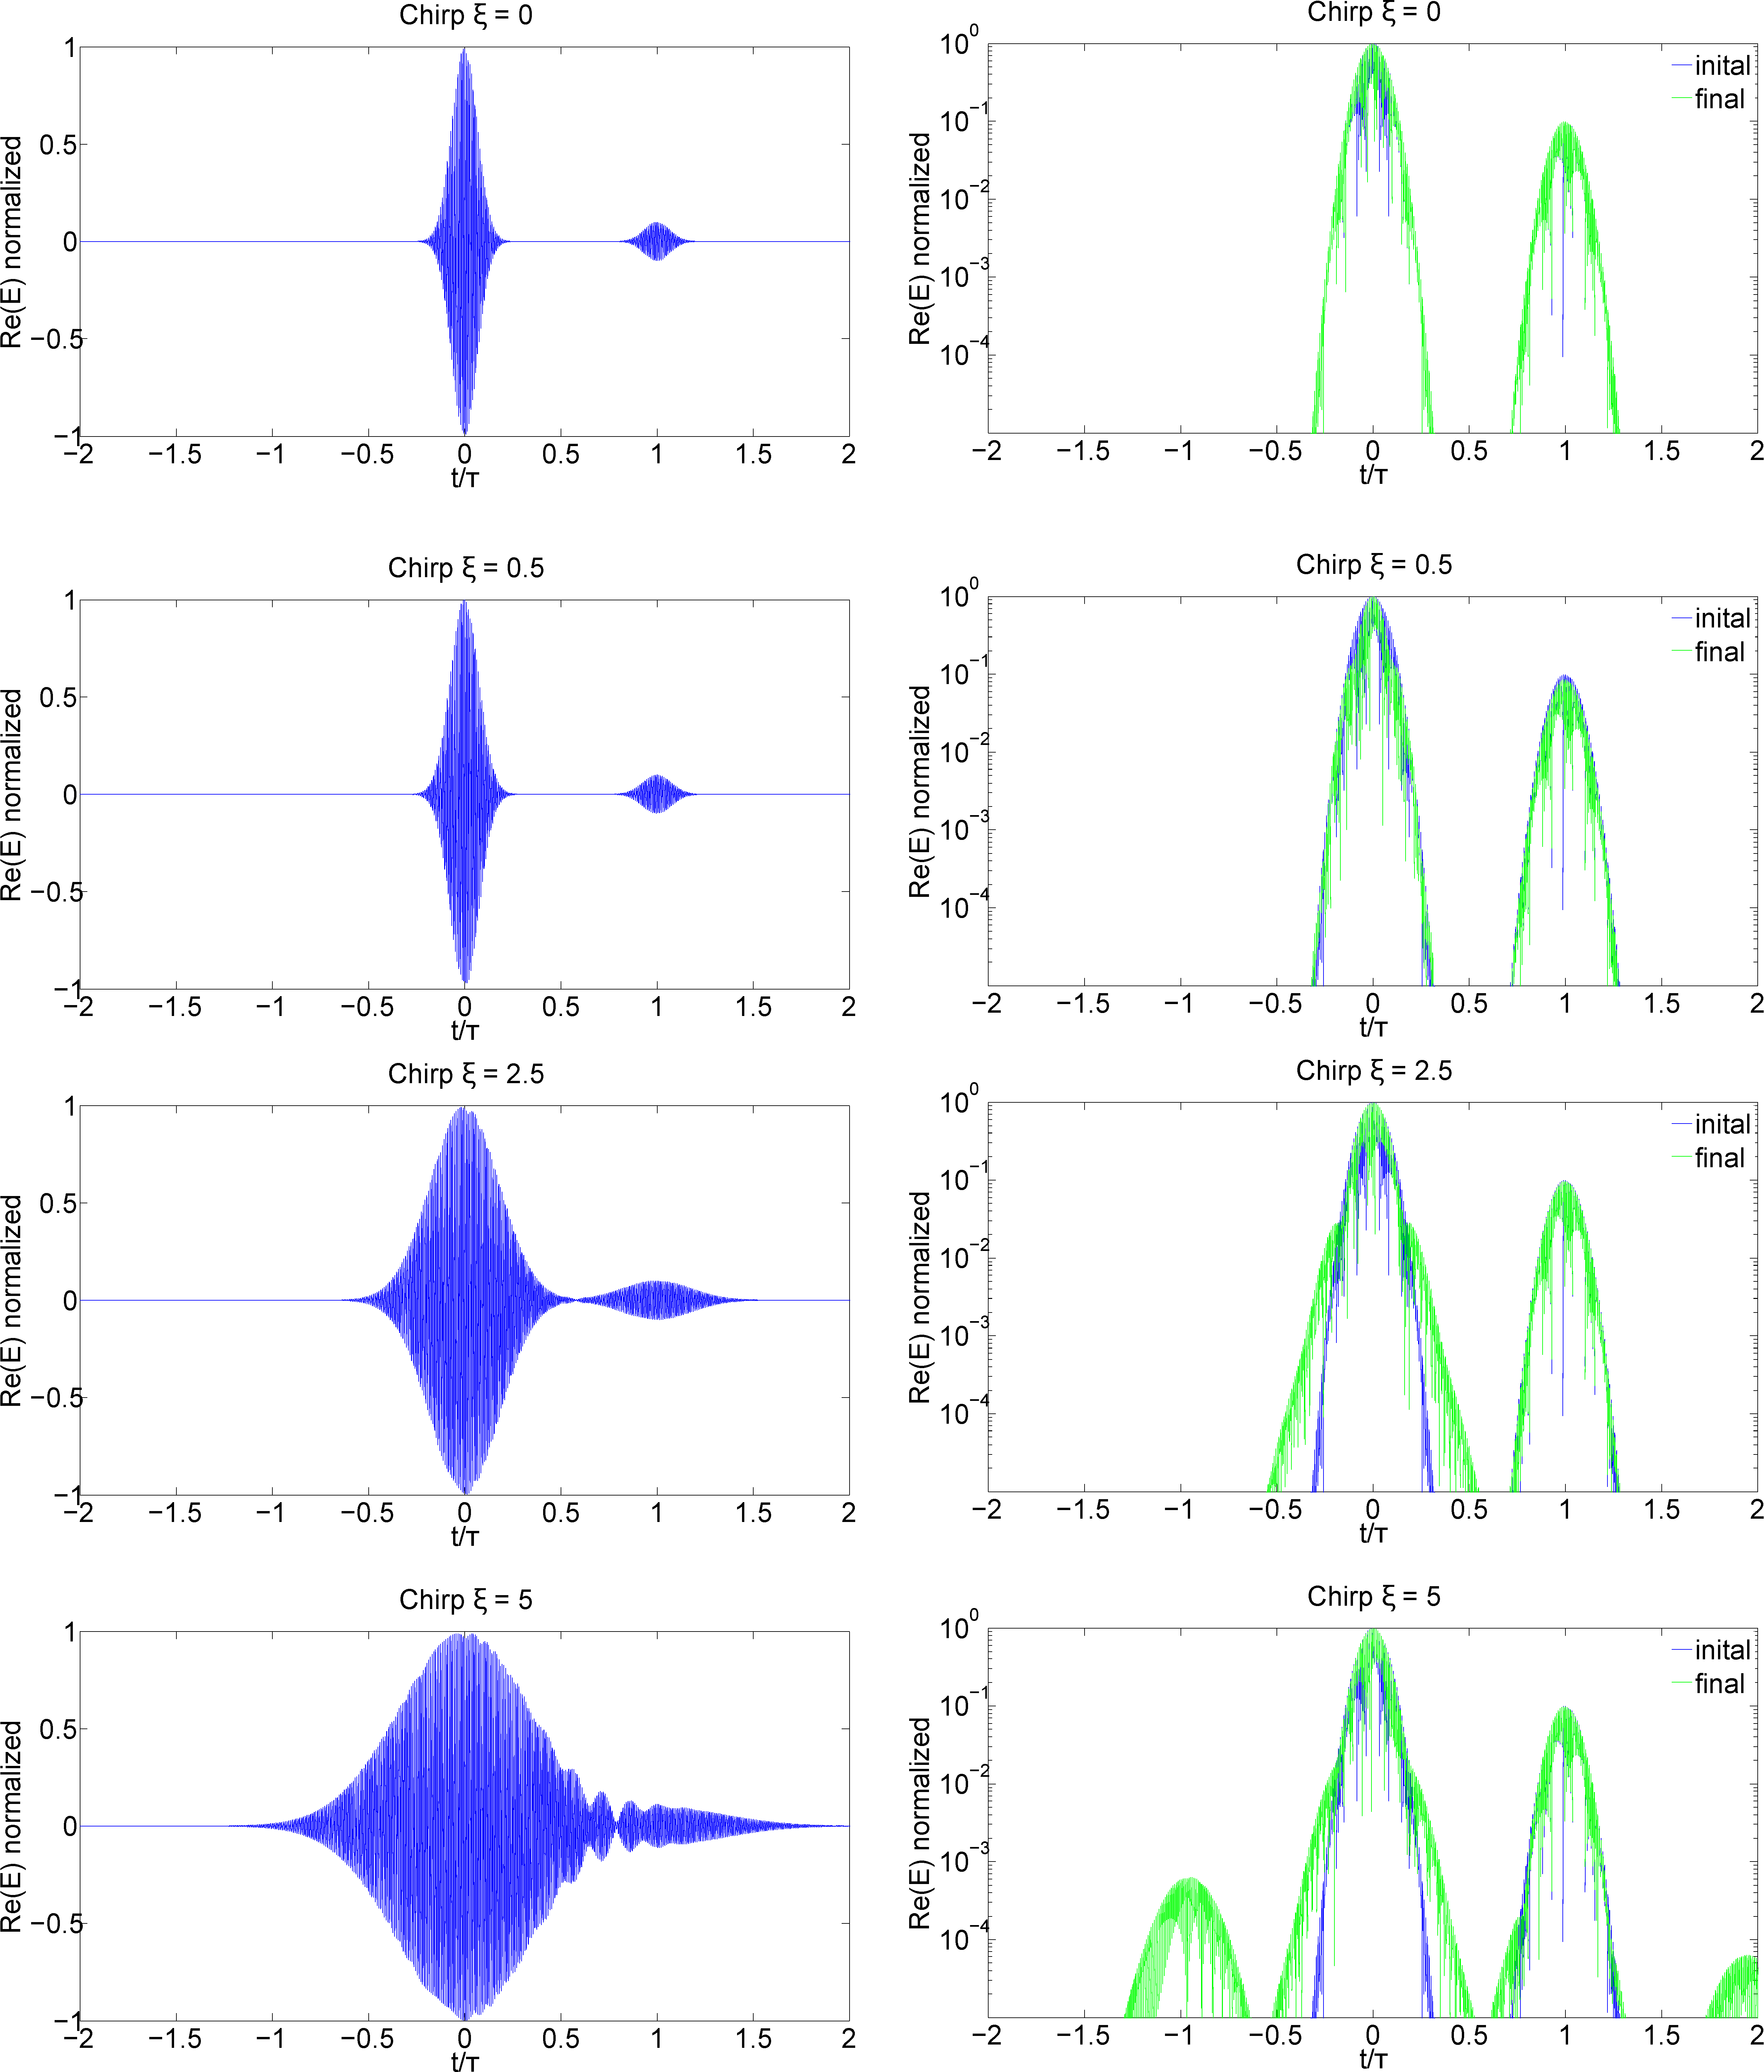
\includegraphics[width =0.8\textwidth]{../chapitre3/images/Result_NL=1.pdf}\\
\caption{\label{fig:Result_NL=1} Influence of SPM on prepulse generation. The left column represents the chirped pulses temporal profile for $\xi = 0 , 0.5 , 2.5$ and $5$ before SPM takes place. The right column shows the temporal profile of the pulses after SPM, and after compression (performed by adding $-\xi$ in spectral domain) on a logarithmic scale. For $\xi = 5$ a prepulse is generated at $t = -\tau$}
\end{figure}

\noindent  Now that we have shown with a simple example the underlying physics behind the postpulse generation, we check we can reproduce this effect using the propagation code \textit{Miró} developed at CEA. Here the size of temporal windows was increased to a few ps to accommodate the experimental duration of the chirped pulse. The input parameters are summarized in the following table:\\

\begin{center}
\begin{tabular}{p{5cm}p{5cm}}
\g{\textit{Miró} input} & \g{value} \\
Temporal window & $-67.5 / +67.5\,\mathrm{ps}$\\
Spatial & N = 1 \\
Duration & 23fs\\
Stretched pulse duration &  45ps \\
Calculation Mode & Phase modulation\\
Peak intensity & $8.9\times 10^{11}\,\mathrm{W/cm^2}$\\
Postpulse delay & 5.3ps\\
Postpulse relative intensity &  $10^{-4}$\\
\end{tabular}
\end{center}



\begin{figure}[H]
\centering
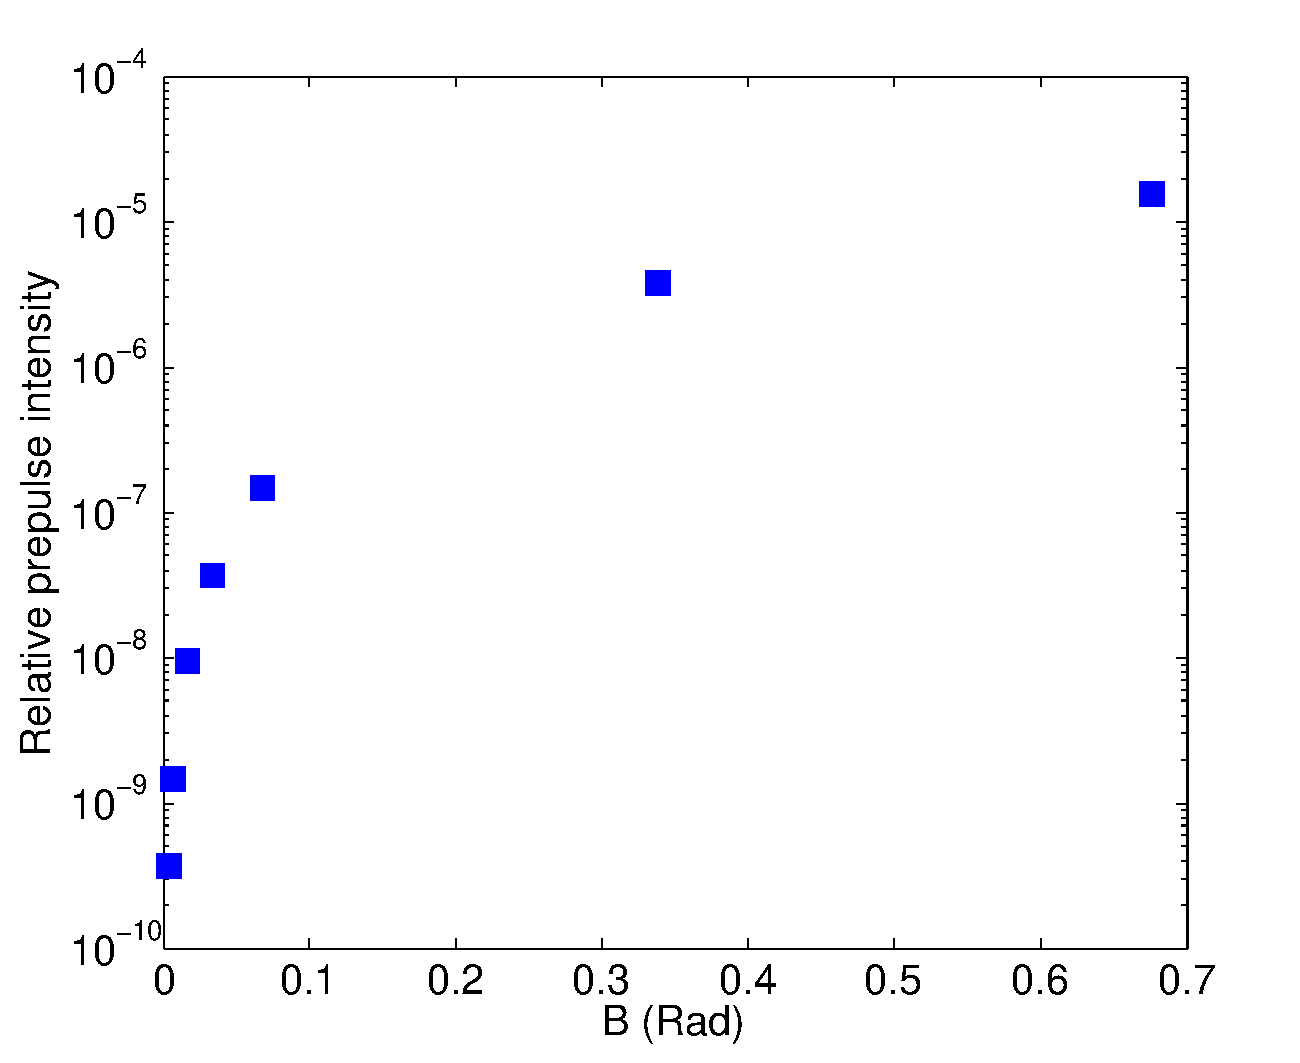
\includegraphics[width =0.9\textwidth]{../chapitre3/images/InfluenceIntegraleB_oneRelativeIntensity.pdf}\\
\caption{\label{fig:InfluenceIntegraleB_oneRelativeIntensity} Result using simulation code \textit{Miró}}
\end{figure}

\noindent  We first ran the simulation by propagating the stretched pulse in an amplifier with a B integral of $0.3\,\mathrm{rad}$ and observed the prepulse formation when both stretched pulses overlapped before amplification. The result was similar (neglecting linear dispersive contribution effects) by replacing the amplifier with a glass plate with identical B integral. This is a further confirmation that prepulse generation from postpulses is due to nonlinear phase distortions, independently of the medium considered. To study the relative conversion efficiency of the process, it was convenient to propagate the pulse into a simple glass plate.
The prepulse relative intensity was retrieved as a function of the B integral and is plotted in Fig~\ref{fig:InfluenceIntegraleB_oneRelativeIntensity}. 



\section{Post-compression and beam shaping}

\begin{figure}[H]
\centering
\makebox[\textwidth][c]{
\includegraphics[width =18cm]{../chapitre3/images/PostComp_chamber.pdf}}\\
\caption{\label{fig:PostComp_chamber} (a) Hollow core fiber setup with active stabilization (b) Prepulse generation using a zero-order broadband beamsplitter reflecting 5 to 10\% of the main pulse. The pump/probe delay is adjusted by translation of a motorized delay stage with sub -$\mathrm{\mu m}$ resolution. (c) Final compression chamber under vacuum ($\sim 10^{-5}\,\mathrm{mBar}$). We compress both main pulse and prepulse on a set of 2 times 4 chirped mirrors introducing $\phi^{(2)} = -250\,\mathrm{fs^2/bounce}$ (\textit{Ultrafast Innovation}). The main pulse can then be attenuated by translating a home-made optical block from a mirror coated to an uncoated surface with $<1\%$ transmission. The main pulse is sent to a 2x telescope and the prepulse 0.5x telescope and both collimated pulses are sent to the experimental chamber to be focused on target}
\end{figure}

As represented in Fig~\ref{fig:femtopower}, after the two amplifiers, the beam is compressed in a set of transmission grisms (\textit{Fastlite}) which have been chosen because they compensate well the third-order phase induced by the stretcher. The beam is then spatially filtered with a 1.5m long hollow core fiber with $260\,\mathrm{\mu m}$ inner diameter. The beam focused into the fiber is projected onto the Bessel propagation modes. \\


\noindent  We used the fiber without any gas inside for spatial filtering and pointing stability: any pointing fluctuation at the fiber input becomes an energy fluctuation at the fiber output. We add an active stabilization of the fiber entrance focus (\textit{Femtolaser}) in closed retraction loop by measuring the far field leaking through the last mirror (M2) with a 4 quadrant photodiode and controlling it with a piezo actuator (M1). The fiber setup is represented in Fig~\ref{fig:PostComp_chamber}(a). \\




\noindent  The beam is divergent at the fiber output so it is recollimated using a $f=1.5$m spherical mirror near normal incidence. Then, the beam is split with an ultrathin broadband beam splitter (\textit{Femtolaser}) to generate a low intensity prepulse, as represented  in Fig~\ref{fig:PostComp_chamber}(b).
The relative delay of the prepulse is adjusted with a translation stage having a 10-cm travel range (minimal increment of $100$nm, specified pitch and yaw $\pm30\,\mathrm{\mu rad}$).\\


\noindent  Both beams are then sent into the so called "compression chamber", a vacuum chamber where they are shaped temporally then spatially. A set of 2" ultrafast chirped mirrors (\textit{Ultrafast Innovation}) is used to compress both beams in copropagating geometry.
The main pulse (much more energetic) can be attenuated by reflecting attenuators mounted on motorized translation stages. This type of optics is represented in Fig~\ref{fig:attenuateur} and was carefully designed to limit the amount of second order phase (GDD) introduced through attenuation. This way, we could perform trustworthy temporal characterization of the attenuated beam by picking up the beam using a motorized flipper mirror.\\

\begin{figure}[H]
\centering
\makebox[\textwidth][c]{
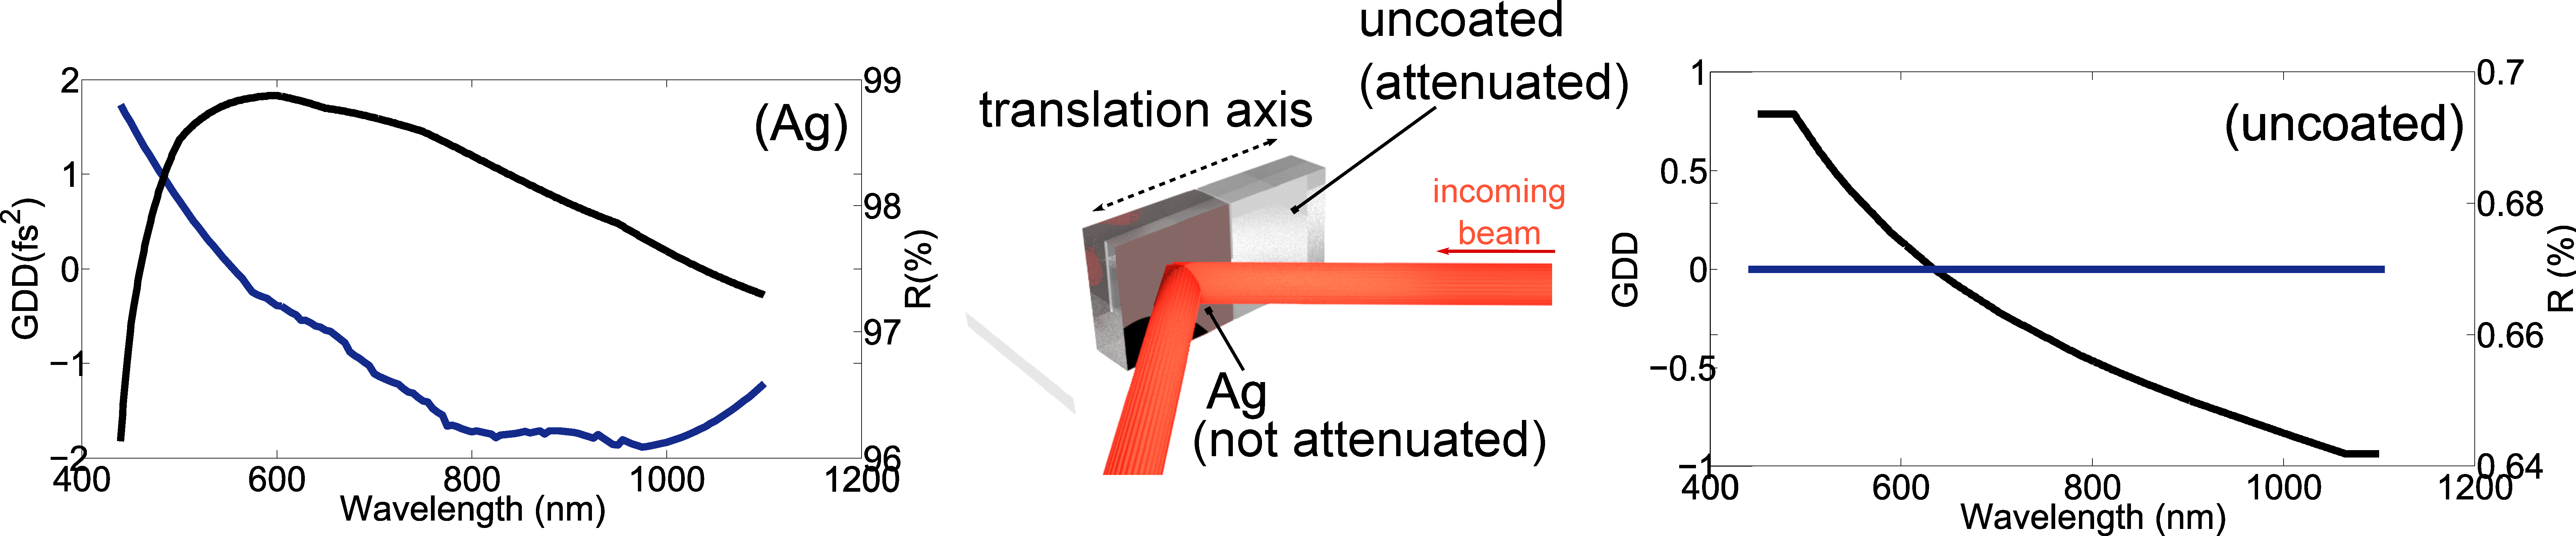
\includegraphics[width =\textwidth]{../chapitre3/images/attenuateur.pdf}}\\
\caption{\label{fig:attenuateur}Attenuator optic: one surface-enhanced Ag-coated (\textit{Femtolaser}), one uncoated bare fused silica surface. Corresponding reflection and GDD are represented}
\end{figure}


\noindent  After the attenuator blocks, the main pulse is sent to a 2x telescope and the prepulse to a 0.5x telescope and both collimated pulses are sent to the experimental chamber to be focused on target as represented in Fig~\ref{fig:PostComp_chamber}(c).
We measured the overall transmission of the hollow-core fiber, the beamsplitter and the propagation inside the compression chamber. Considering this, we enter the experimental chamber with a $30$mm, $23$fs, 3mJ compressed pulse, and a prepulse of 7mm, $\sim 50\,\mathrm{\mu J}$ also compressed to 23fs.
The spatial profile at the focus of the off axis parabola is measured and the beam is attenuated by inserting a motorized microscope objective sending the magnified image of the focus on a CCD camera place outside the vacuum chamber. 





\section{Solid-target experimental setup}
\label{section:Solid target experimental set-up}

\subsection{Experimental chamber and beam profile}

\begin{figure}[H]
\centering
\makebox[\textwidth][c]{
\includegraphics[width =18cm]{../chapitre3/images/SolidTargetChamber.pdf}}\\
\caption{\label{fig:SolidTargetChamber} Experimental setup of pump/probe experiment on solid target at a 1kHz laser repetition rate}
\end{figure}



The experimental setup is represented in Fig~\ref{fig:SolidTargetChamber}. Details of the different diagnostics installed for electrons and harmonic detection will be given in the following chapters. Here, the 30fs, 3mJ  800nm main pulse exiting the compression chamber enters the interaction chamber and is focused with a f/1.2  off axis parabola mounted on a translation stage used for controlled defocusing. The focusing plane of the parabola is carefully aligned with the solid-target plane. The prepulse is focused using the same parabola to facilitate alignment and minimize pump/probe temporal jitter. To do so, a 8mm hole was made in the last mirror M1 to make both beams collinear prior to the focusing parabola.
Using the attenuators installed in the compression chamber (previously described in Fig~\ref{fig:PostComp_chamber}), the profile of the beam at focus is recorded with a CCD camera placed outside vacuum: to image the focus, we simply need to translate the target holder to align the microscope objective with the optical axis defined after the parabola with no need to break the vacuum in the chamber. In Fig~\ref{fig:Focus} we represent the spatial profile of the main pulse (a) and the prepulse (c) at the focus of the parabola. We could also bypass the telescope to decrease the beam aperture, which ultimately increases the focus spot size by a factor~$\sim 2$.


\begin{figure}[H]
\centering
\makebox[\textwidth][c]{
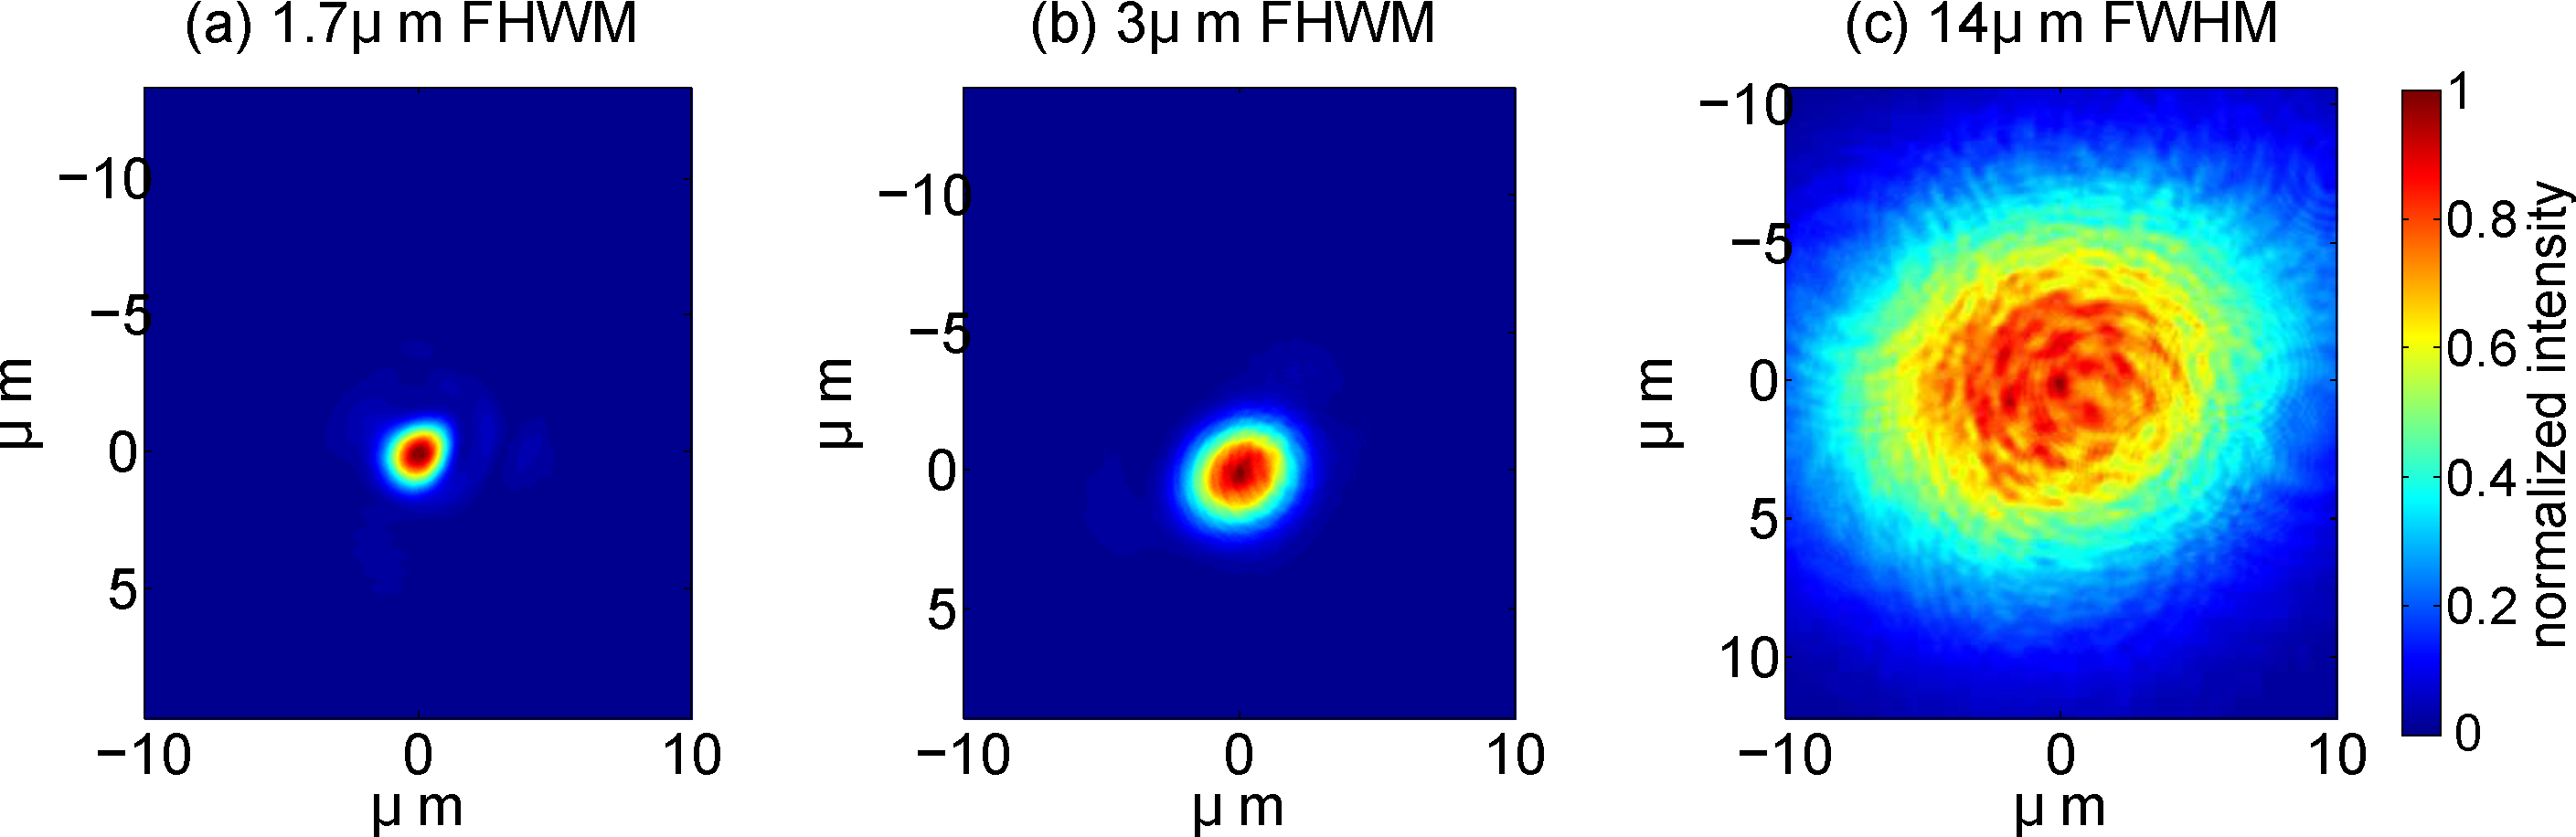
\includegraphics[width =\textwidth]{../chapitre3/images/Focus.pdf}}\\
\caption{\label{fig:Focus}Profile recorded at the focus of the parabola (a) Beam expander in the compression chamber (b) Bypassing the beam expander (c) Prepulse profile}
\end{figure}

\subsection{Beam temporal profile}

The temporal profile of the main pulse is measured after the attenuator with a Wizzler (\textit{Fastlite}). Two crossed polarized and delayed replicas of the pulse are generated using a Calcite plate and sent to a $BaF_2$ crystal where the most intense pulse creates a crossed polarized replica through XPW. This XPW reference beam interfers with the first replica which creates spectral fringes. Using a well-suited retrieval algorithm, it is possible to reconstruct both the spectrum and phase of the initial beam. This is illustrated in Fig~\ref{fig:PWizzler_20150401} where we performed a Wizzler measurement for the compressed pulse with or without apodization of the spectrum using the Dazzler (cf section~\ref{subsection:Spectral clipping}).

\begin{figure}[H]
\centering
\makebox[\textwidth][c]{
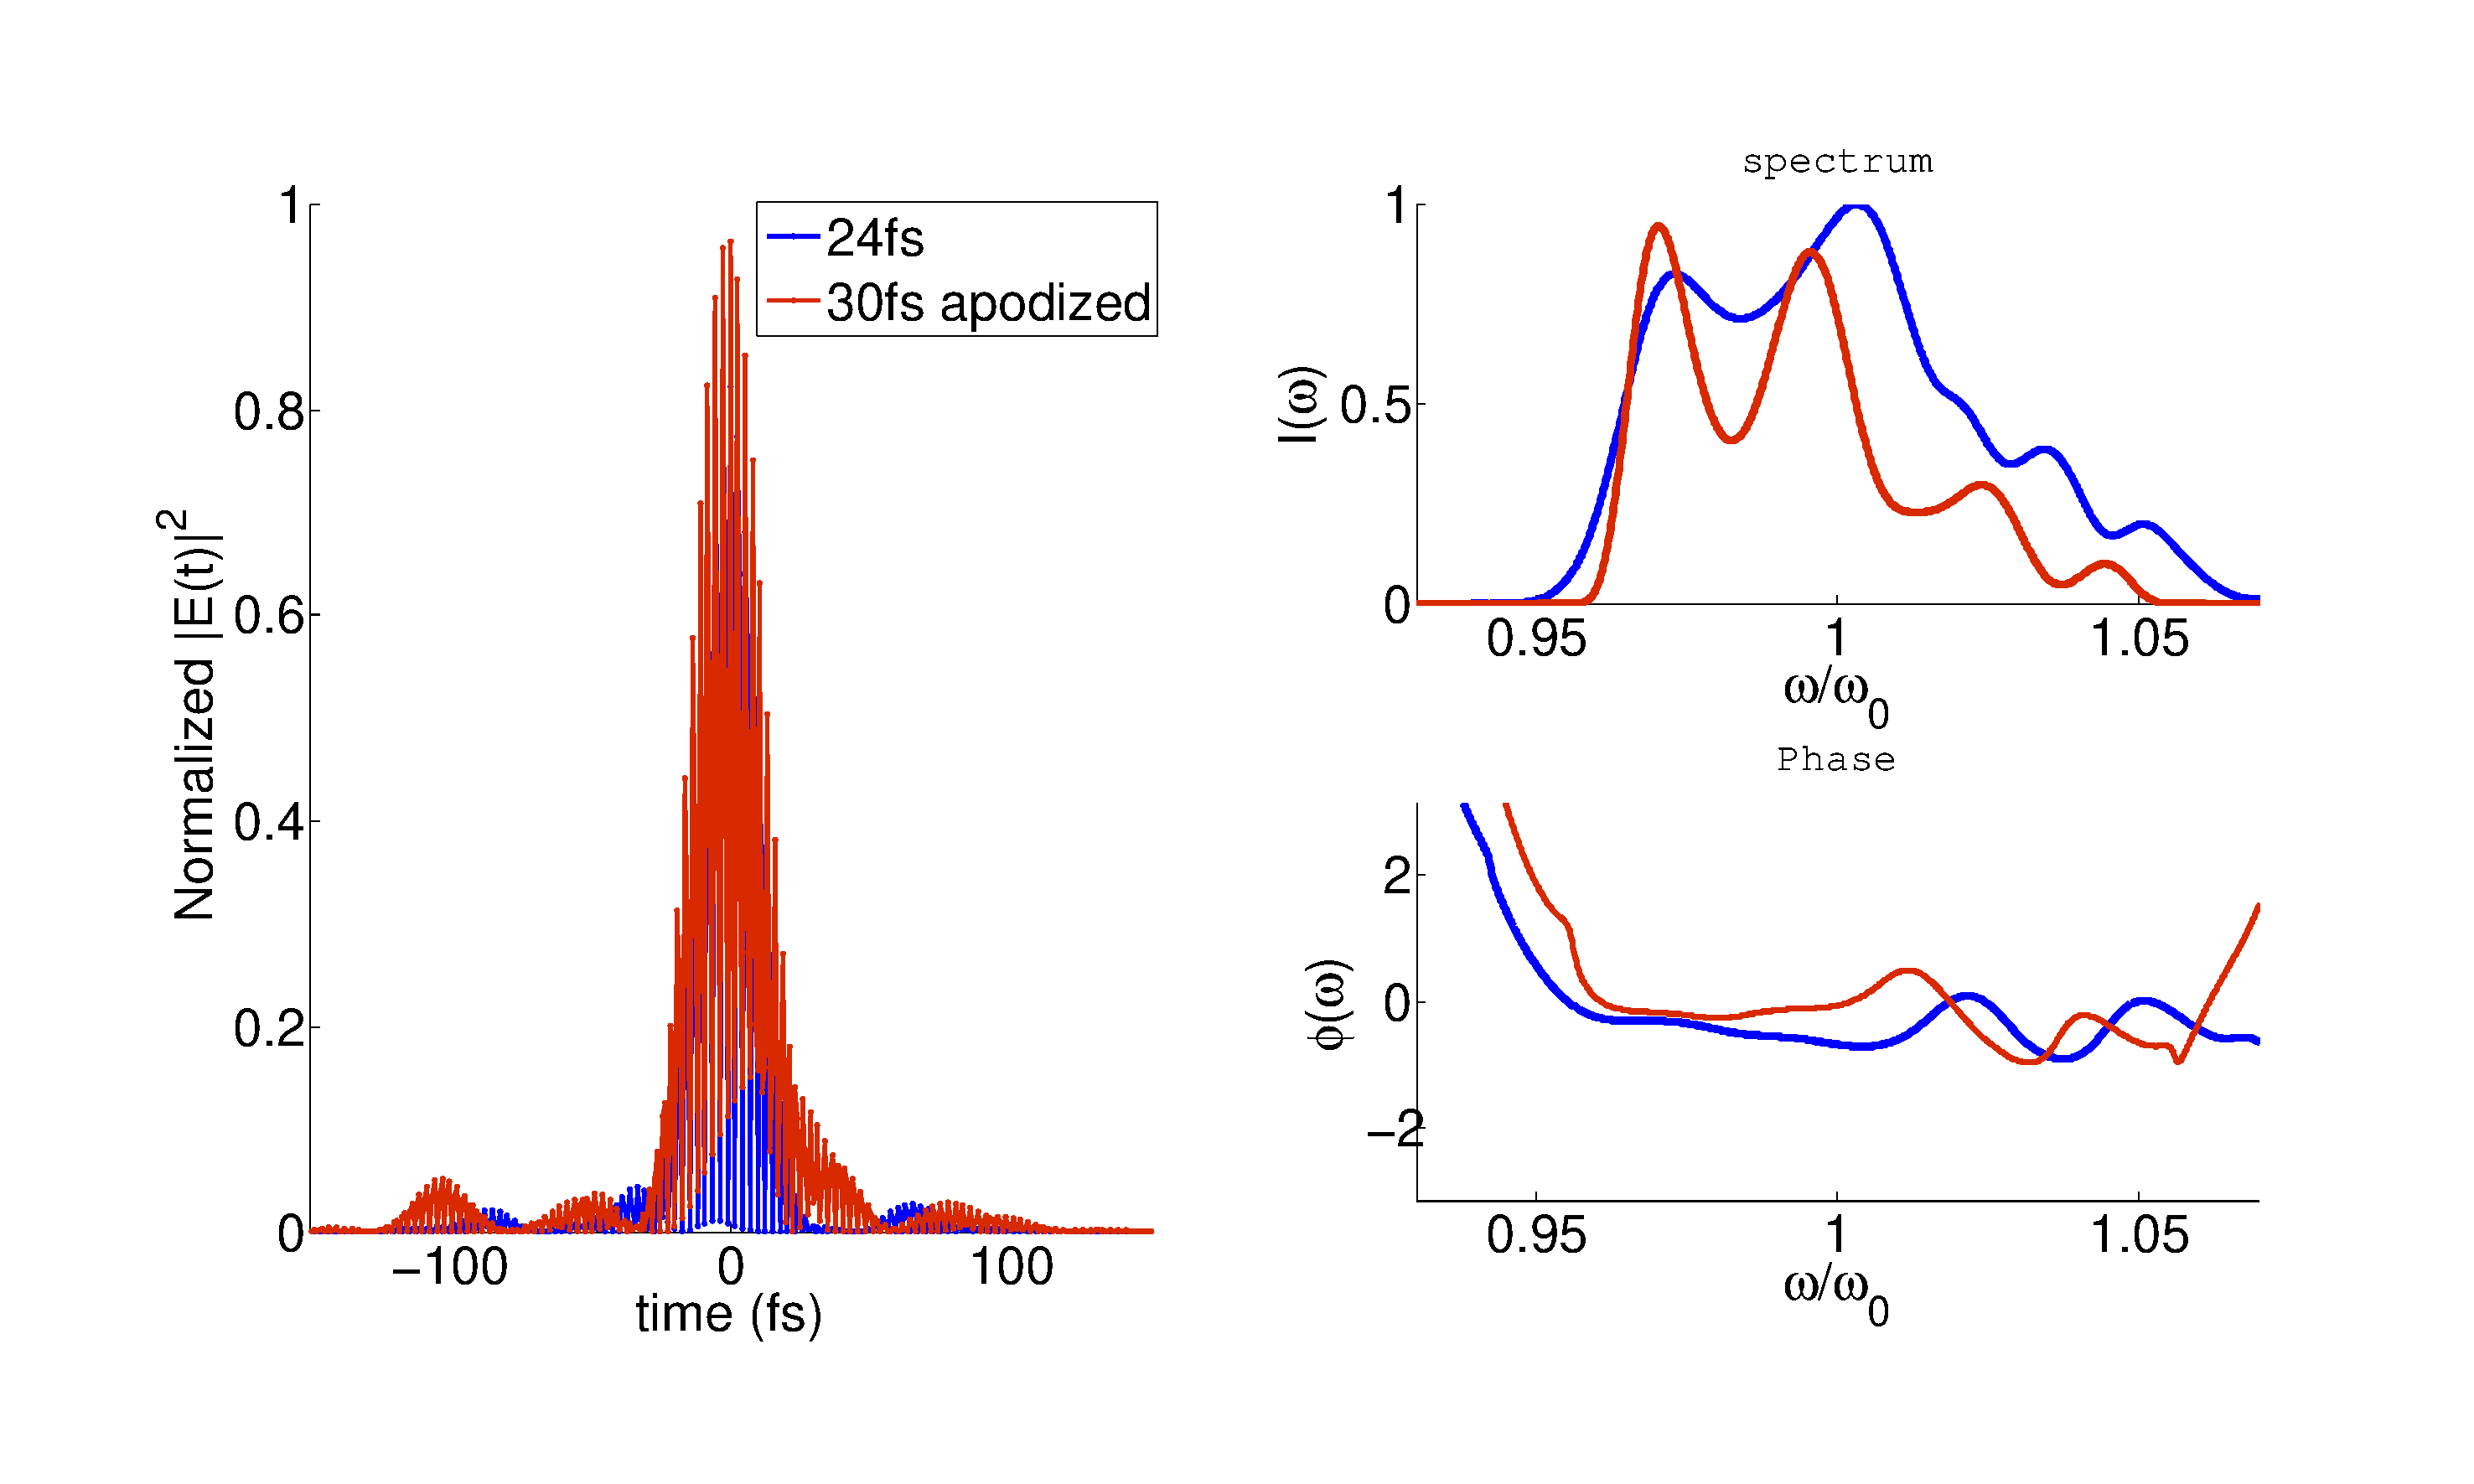
\includegraphics[width =\textwidth]{../chapitre3/images/Wizzler_20150401-square.pdf}}\\
\caption{\label{fig:PWizzler_20150401} Wizzler measurement before the interaction for compressed $24$fs pulse (blue curve) and when apodizing the spectrum to improve the laser contrast (red curve), resulting in an increase to 30fs. On left caption, we represent the square of the real part modulus of the field in both cases.}
\end{figure}

\noindent  On the femtosecond scale, no net difference can be observed between the non-apodized and the apodized pulse except that the latter has a longer pulse duration (30fs as opposed to 24fs). The clear advantage of spectral apodization has been described in~\ref{subsection:Spectral clipping} and relates to the ps coherent contrast. However, the measurement from Fig~\ref{fig:PWizzler_20150401} shows that the spectral modulations combined with the residual spectral phase of the beam will result in the generation of satellite pulses on the femtosecond time scale, and with intensities $\sim 5\mathrm{\%}$ that of the main pulse. This is enough to initiate High Harmonic Generation and therefore, generate a complex structure of harmonics with spectral modulations $\Delta \omega$, which we can evaluate to be of the order of:

$$
\Delta \omega / \omega_0 \sim 0.05-0.3
$$

\noindent This is typical of what we can observe experimentally on our harmonics spectra, especially for increased intensities.

\subsection{kHz solid target}

In order to perform solid-target experiments at 1kHz, the surface of the target has to be refreshed every millisecond. In many low-repetition-rate laser facilities, the standard method to refresh the target consists in translating a solid bulk material after every shot\cite{kahaly2013direct}. In our case, 
the target is a 4 inch cylindrical fused silica wafer optically polished to $\lambda/20$ surface flatness and mounted on a rotation axis with adjustable rotation speed \cite{borot2011high}. Typically, we set the rotation speed to $\sim 9 \,\mathrm{rad/s}$ in order to separate each successive shot by at least $\sim 100\,\mathrm{\mu m}$ to account for the damage extent (the focus is only a few microns large) as illustrated by Fig~\ref{fig:ImpactTarget}.

\begin{figure}[H]
\centering
\makebox[0.9\textwidth][c]{
\includegraphics[width =0.82\textwidth]{../chapitre3/images/ImpactTarget.pdf}}\\
\caption{\label{fig:ImpactTarget} Solid-target surface after an experiment visualized with an optical microscope (a) Shots on fused silica where shot overlap is due to the low target rotation velocity (b) Shots on fused silica with correct spacing
(c) Shots on plastic with correct spacing where different impact sizes correspond to different laser energies}
\end{figure}


\noindent  Before running the experiment, we align very precisely the target plane normal to the rotating axis using 3 piezo actuators and minimize the horizontal and vertical angular fluctuations $\alpha_x$ and $\alpha_y$ down to $50\,\mathrm{\mu rad}$(mechanical limit). The measurement of these angular fluctuations as well as the depth variation is done interferometrically using a stabilized He-Ne sent inside a Mach Zehnder interferometer in that horizontal plane, and following the interference pattern as the target is rotating. This alignment procedure, represented in Fig~\ref{fig:TargetStabilization}, is essential to ensure the good reproducibility of our experiment: the depth fluctuations of the target surface should be inferior to the  Rayleigh length of the focused beam, which is $\sim \mathrm{2\mu m}$. 
On Fig~\ref{fig:TargetStabilization}(e), $d$ is retrieved as a function of target revolution with peak-to-valley values $\sim 1 \,\mathrm{\mu m}$ which is good enough to run an experiment.

\begin{figure}[H]
\centering
\makebox[\textwidth][c]{
\includegraphics[width =\textwidth]{../chapitre3/images/TargetStabilization.pdf}}\\
\caption{\label{fig:TargetStabilization} Target stabilization setup (a) Reference fringes when the target is not rotating  (b) Effect of horizontal phase corresponding to angle $\alpha_x$ variation resulting in fringes spacing (c) Effect of vertical phase corresponding to angle $\alpha_y$ variations resulting in a tilt of the fringes (d) Effect of constant phase shift corresponding to depth fluctuations: translation of the fringes (e) Retrieved $\alpha_x$, $\alpha_y$ and depth $d$ when target is rotating}
\end{figure}





\section{Conclusion}

In this section, we have presented the overall architecture of our double CPA system, which delivers a few mJ, sub-30fs pulses at a 1 kHz repetition rate to our experimental chamber. In our solid-target experiment, controlling the laser temporal contrast is crucial to prevent destruction of the target by a pedestal, which is why there is an XPW contrast filter between the two CPA units. However, filtering the contrast alone is not enough to ensure the absence of prepulses. One must also prevent postpulses from forming before stretching the pulse to picosecond durations to avoid nonlinear prepulse creation. Finally, the experiments which will be presented in this manuscript are possible thanks to the solid-target stability and the possibility to refresh the target surface every millisecond. This way, we accumulate  hundred of shots on our detectors, enabling good  interaction statistics.





























